\section{Basic Concepts}

\paragraph{All About Grassman Variables}
Grassman variables $\theta_{i}$ are defined such that multiplication of two different variables anticommutes. This means that all functions of a set of Grassman variables can be written as
\begin{align*}
	F(\theta) = \sum\limits_{i = 0}^{n}\frac{1}{i!}A^{(i), j_{1}\dots j_{i}}\theta_{j_{1}}\dots\theta_{j_{i}},
\end{align*}
with summation over the indices $j$. The coefficients $A$ are completely antisymmetric.

Functions of Grassman numbers are defined as even $A^{k} = 0$ for all even $k$ and similarly for odd functions. This implies that $FG = GF$ if either is even and $FG = -GF$ otherwise.

We define derivatives with respect to Grassman variables as
\begin{align*}
	\pdv{\theta_{i}}(\theta_{j}) = \delta_{ij}.
\end{align*}
These derivatives anticommute. They satisfy the product rule
\begin{align*}
	\pdv{\theta_{i}}(FG) = \pdv{F}{\theta_{i}}{G} + (-1)^{\abs{F}}F\pdv{G}{\theta_{i}},
\end{align*}
where $\abs{F}$ is $1$ if $F$ is even and $0$ if $F$ is odd. Note that this implies the sign convention
\begin{align*}
	\pdv{\theta_{i}}\theta_{i}\theta_{j} = -\pdv{\theta_{i}}\theta_{j}\theta_{i}.
\end{align*}
For a composite function
\begin{align*}
	f(G(\theta)) &= \sum\limits_{n}f_{n}G^{n}(\theta),
\end{align*}
the chain rule
\begin{align*}
	\pdv{\theta_{i}} f(G(\theta)) &= \pdv{G}{\theta_{i}}\dv{f}{G}
\end{align*}
also applies.

Integrals over Grassman variables are defined according to
\begin{align*}
	\inte{}{}\dd{\theta_{i}} = 0,\ \inte{}{}\dd{\theta_{i}}\theta_{j} = \delta_{ij}.
\end{align*}
This has the peculiar consequence
\begin{align*}
	\inte{}{}\dd{\theta_{i}}F(\theta) = \pdv{F}{\theta_{i}}.
\end{align*}
We know that all functions of Grassman variables can be factorized as $F(\theta) = A(\theta) + \theta_{i}B(\theta)$, where neither $A$ nor $B$ depend on $\theta_{i}$. This has the consequence that shifts in any one variable does not affect the integral. Scaling of variables does not work that way, however, as we saw that differentiation and integration has the same effect. This produces the general result
\begin{align*}
	\theta_{j} = A_{ij}\phi_{j}\implies \dd{\theta}_{1}\dots\dd{\theta}_{n} = \frac{1}{\det(A)}\dd{\phi}_{1}\dots\dd{\phi}_{n}.
\end{align*}

The Dirac delta function is defined in this context such that it obeys the relation
\begin{align*}
	\inte{}{}\dd{\theta}_{i}F(\theta)\delta(\theta_{i}) = \eval{F}_{\theta_{i} = 0}.
\end{align*}
From what we have above we see that $\delta(\theta_{i}) = \theta_{i}$ satisfies this. This again has consequences of scaling the Dirac delta being different - more specifically
\begin{align*}
	\prod\limits_{i}\delta(A_{ij}\delta_{j}) = \det(A)\prod\limits_{i}\delta(\delta_{i}).
\end{align*}

Complex Grassman variables can also be defined according to
\begin{align*}
	\theta_{k} = \phi(k) + i\psi(k).
\end{align*}
Using the relations above we find
\begin{align*}
	\dd{\theta}_{k}\dd{\theta}_{k}\cc = i\dd{\phi}_{k}\dd{\psi}_{k}.
\end{align*}
%TODO: Show thing with Gaussian

\paragraph{The Path Integral Approach}
We will now switch from canonical quantization to path integrals as our basis for quantum field theory. This has a few advantages:
\begin{itemize}
	\item It switches from the Hamiltonian to the Lagrangian, which can more easily be manifestly Lorentz invariant.
	\item The switch to the Lagrangian allows for more aesthetic handling of Lagrangians with field derivatives.
	\item It allows for better handling of non-Abelian gauge theories.
\end{itemize}

\paragraph{Path Integrals in Quantum Mechanics}
Consider a system with Lagrangian
\begin{align*}
	\ham = \frac{p^{2}}{2m} + V(q).
\end{align*}
In the Heisenberg pictures, the $q$ operator is given by
\begin{align*}
	q(t) = e^{i\ham t}q(0)e^{-i\ham t},
\end{align*}
We study states of the form $\ket{q, t}$, which are eigenstates of $q(t)$ with eigenvalue $q$. We note that
\begin{align*}
	q(t)e^{i\ham t}\ket{q} = e^{i\ham t}qe^{-i\ham t}e^{i\ham t}\ket{q} = qe^{i\ham t}\ket{q},
\end{align*}
hence this is the form of the states we are considering. Eigenstates at reference time $t\p$ will be implicitly labelled when convenient.

We might consider the amplitude of the system evolving from $q\p$ to $q^{\prime\prime}$ over some time. This is given by
\begin{align*}
	\braket{q^{\prime\prime}, t^{\prime\prime}}{q\p, t\p} = \mel{q^{\prime\prime}}{e^{-i\ham(t^{\prime\prime} - t\p)}}{q\p},
\end{align*}
which coincides with the expression in the Schrödinger picture. To introduce the path integral we will discretize the time interval into $N$ slices of width $\Delta$ and write
\begin{align*}
	\mel{q^{\prime\prime}}{e^{-i\ham(t^{\prime\prime} - t\p)}}{q\p} = \mel{q^{\prime\prime}}{e^{-i\ham\Delta}\dots e^{-i\ham\Delta}}{q\p}.
\end{align*}
Between each pair of time evolution operators we now place a completeness relation, reducing the problem to computing
\begin{align*}
	\mel{q_{i + 1}}{e^{-i\ham\Delta}}{q_{i}}.
\end{align*}
The final value of the amplitude will be the product of all such factors from $0$ to $N$. We can now split the exponentials according to
\begin{align*}
	\mel{q_{i + 1}}{e^{-i\ham\Delta}}{q_{i}} = \mel{q_{i + 1}}{e^{-i\Delta\frac{p^{2}}{2m}}e^{-i\Delta V(q)}e^{-\frac{1}{2}\Delta^{2}\comm{\frac{p^{2}}{2m}}{V(q)}}\dots}{q_{i}}.
\end{align*}
Due to our discretization we may now ignore the higher-order factors, leaving
\begin{align*}
	\mel{q_{i + 1}}{e^{-i\ham\Delta}}{q_{i}} = \mel{q_{i + 1}}{e^{-i\Delta\frac{p^{2}}{2m}}e^{-i\Delta V(q)}}{q_{i}}.
\end{align*}
The first factor is easily dealt with. To handle the second, we introduce a new completeness relation such that
\begin{align*}
	\mel{q_{i + 1}}{e^{-i\ham\Delta}}{q_{i}} &= e^{-i\Delta V(q_{i})}\integ{}{}{p}\mel{q_{i + 1}}{e^{-i\Delta\frac{p^{2}}{2m}}}{p}\braket{p}{q_{i}} \\
	                                         &= e^{-i\Delta V(q_{i})}\integ{}{}{p}e^{-i\Delta\frac{p^{2}}{2m}}\braket{q_{i + 1}}{p}\braket{p}{q_{i}} \\
	                                         &= e^{-i\Delta V(q_{i})}\integ{}{}{p}e^{-i\Delta\frac{p^{2}}{2m} + ip(q_{i + 1} - q_{i})} \\
	                                         &= e^{-i\Delta V(q_{i})}\integ{}{}{p}e^{-i\frac{\Delta}{2m}\left(p - \frac{m}{\Delta}(q_{i + 1} - q_{i})\right)^{2}}e^{i\frac{m\Delta}{2}\left(\frac{q_{i + 1} - q_{i}}{\Delta}\right)^{2}} \\
	                                         &= e^{i\Delta\left(\frac{1}{2}m\left(\frac{q_{i + 1} - q_{i}}{\Delta}\right)^{2} - V(q_{i})\right)}\integ{}{}{p}e^{-i\frac{\Delta}{2m}\left(p - \frac{m}{\Delta}(q_{i + 1} - q_{i})\right)^{2}}
\end{align*}
We will leave the integral as is, as it merely provides some normalization factor in the end. Dubbing it $A$ we find
\begin{align*}
	\braket{q^{\prime\prime}, t^{\prime\prime}}{q\p, t\p} &= \inte{}{}\dd{q}_{1}\dots\dd{q}_{N}A^{N}e^{i\Delta\left(\frac{1}{2}m\left(\frac{q_{1} - q\p}{\Delta}\right)^{2} - V(q\p)\right)}\dots e^{i\Delta\left(\frac{1}{2}m\left(\frac{q^{\prime\prime} - q_{N}}{\Delta}\right)^{2} - V(q_{N})\right)} \\
	                                                      &= \inte{}{}\dd{q}_{1}\dots\dd{q}_{N}A^{N}e^{i\sum\limits_{i = 0}^{N}\Delta\left(\frac{1}{2}m\left(\frac{q_{i + 1} - q_{i}}{\Delta}\right)^{2} - V(q_{i})\right)}.
\end{align*}
Now comes the kicker: We let $N$ go to infinity and $\Delta$ to zero such that the sum in the exponent goes to an integral. In this limit we see that what is left is in fact the integral of the Lagrangian, or the action. The action of what, you ask? It's the action corresponding to a particular choice of all the intermediate $q$.

The integration over an infinite set of such intermediate values corresponds to an integral over function space - over all possible functional forms of $q(t)$. This is what is termed the path integral. It is generally denoted as
\begin{align*}
	\pinte{}{x}.
\end{align*}
Renaming the normalization constant we therefore have
\begin{align*}
	\braket{q^{\prime\prime}, t^{\prime\prime}}{q\p, t\p} &= C\pinte{}{q}e^{iS}.
\end{align*}

One might ask whether the limit that defines the path integral really exists. Yes, one might very well ask that.

\paragraph{Observables from Path Integrals}
Let us now consider
\begin{align*}
	\mel{q^{\prime\prime}, t^{\prime\prime}}{\torp q(t_{n})\dots q(t_{1})}{q\p, t\p}.
\end{align*}
We may consider the times to be correctly ordered for convenience, allowing us to remove the time ordering. Discretizing time and taking $t_{i} - t\p = k_{i}\Delta$ we can write
\begin{align*}
	q(t_{i + 1})q(t_{i}) &= e^{i\ham k_{i + 1}\Delta}qe^{-i\ham k_{i + 1}\Delta}e^{i\ham k_{i}\Delta}qe^{-i\ham k_{i}\Delta} = e^{i\ham k_{i + 1}\Delta}qe^{-i\ham (k_{i + 1} - k_{i})\Delta}qe^{-i\ham k_{i}\Delta}.
\end{align*}
Using completeness we have
\begin{align*}
	e^{-i\ham (k_{i + 1} - k_{i})\Delta} = \inte{}{}\dd{q_{k_{i } + 1}}\dots\dd{q_{k_{i + 1}}}\op{q_{k_{i + 1}}}e^{-i\ham \Delta}\dots\op{q_{k_{i} + 1}}e^{-i\ham \Delta},
\end{align*}
hence
\begin{align*}
	q(t_{i + 1})q(t_{i}) &= \inte{}{}\dd{q_{k_{i } + 1}}\dots\dd{q_{k_{i + 1}}}e^{i\ham k_{i + 1}\Delta}q\op{q_{k_{i + 1}}}e^{-i\ham \Delta}\dots\op{q_{k_{i} + 1}}e^{-i\ham \Delta}qe^{-i\ham k_{i}\Delta} \\
	                     &= \inte{}{}\dd{q_{k_{i } + 1}}\dots\dd{q_{k_{i + 1}}}q_{k_{i + 1}}e^{i\ham k_{i + 1}\Delta}\op{q_{k_{i + 1}}}e^{-i\ham \Delta}\dots\op{q_{k_{i} + 1}}e^{-i\ham \Delta}qe^{-i\ham k_{i}\Delta}.
\end{align*}
On the left end we pair up $e^{-i\ham N\Delta}$ with $e^{i\ham k_{n}\Delta}$ and on the right end no modifications are needed, hence
\begin{align*}
	\mel{q^{\prime\prime}, t^{\prime\prime}}{\torp q(t_{n})\dots q(t_{1})}{q\p, t\p} &= \inte{}{}\dd{q_{1}}\dots\dd{q_{N}}q_{k_{1}}\dots q_{k_{n}}\mel{q^{\prime\prime}}{e^{-i\ham \Delta}}{q_{N}}\dots \mel{q_{1}}{e^{-i\ham \Delta}}{q\p}.
\end{align*}
We can now recognize results from previously, and in the limit of infinitely fine discretization we obtain
\begin{align*}
	\mel{q^{\prime\prime}, t^{\prime\prime}}{\torp q(t_{n})\dots q(t_{1})}{q\p, t\p} = C\pinte{}{q}q(t_{n})\dots q(t_{1})e^{iS}.
\end{align*}
Note that the ordering in the integration is no longer important.

%TODO: Show
As a side note, an ad hoc argument for why the path integral converges can be found by going back to the discrete variant, performing a Wick rotation of the time step $\Delta$ and thus show that the amplitude of the contributions diverges exponentially as one strays from the path of least action.

\paragraph{Green's Functions from Path Integrals}
We can use the above to obtain the Green's function from path integrals. We recall that the Green's function is defined as
\begin{align*}
	G(t_{1}, \dots, t_{n}) = \frac{\expval{\torp q(t_{1})\dots q(t_{n})}{\Omega}}{\braket{\Omega}}.
\end{align*}
Here we  will use $t = 0$ as our reference. To get an expression in terms of the ground state we use completion to write
\begin{align*}
	\mel{q^{\prime\prime}, t^{\prime\prime}}{\torp q(t_{n})\dots q(t_{1})}{q\p, t\p} &= \sum\limits_{n, m}\mel{q^{\prime\prime}}{e^{-i\ham t^{\prime\prime}}}{n}\mel{n}{\torp q(t_{n})\dots q(t_{1})}{m}\mel{m}{e^{i\ham t\p}}{q\p} \\
	&= \sum\limits_{n, m}e^{i(E_{m}t\p - E_{n}t^{\prime\prime})}\braket{q^{\prime\prime}}{n}\mel{n}{\torp q(t_{n})\dots q(t_{1})}{m}\braket{m}{q\p}.
\end{align*}
We will now consider the limit of large times (which is what is relevant for QFT contexts anyway). We will also extend time to be complex. In summary we write
\begin{align*}
	t\p = -\tau(1 - i\varepsilon),\ t^{\prime\prime} = \tau(1 - i\varepsilon),
\end{align*}
where we take $\tau$ to be large and let $\varepsilon\to 0$ at the end of our calculations. Thus we have
\begin{align*}
	\mel{q^{\prime\prime}, t^{\prime\prime}}{\torp q(t_{n})\dots q(t_{1})}{q\p, t\p} &= \sum\limits_{n, m}e^{-i\tau(1 - i\varepsilon)(E_{m} + E_{n})}\braket{q^{\prime\prime}}{n}\mel{n}{\torp q(t_{n})\dots q(t_{1})}{m}\braket{m}{q\p} \\
	&= \sum\limits_{n, m}e^{-i\tau(E_{m} + E_{n})}e^{-\tau\varepsilon(E_{m} + E_{n})}\braket{q^{\prime\prime}}{n}\mel{n}{\torp q(t_{n})\dots q(t_{1})}{m}\braket{m}{q\p}.
\end{align*}
In the limit of large times the only contribution thus comes from the ground state, and we have
\begin{align*}
	\mel{q^{\prime\prime}, t^{\prime\prime}}{\torp q(t_{n})\dots q(t_{1})}{q\p, t\p} &= \braket{q^{\prime\prime}}{\Omega}\braket{\Omega}{q\p}\mel{\Omega}{\torp q(t_{n})\dots q(t_{1})}{\Omega}.
\end{align*}
The left-hand side is now a path integral and the right-hand side is proportional to the Green's function. We thus have
\begin{align*}
	G(t_{1}, \dots, t_{n}) = \frac{\pinte{}{q}q(t_{n})\dots q(t_{1})e^{iS}}{\pinte{}{q}e^{iS}}.
\end{align*}

\paragraph{Path Integrals in Field Theories}
In moving to field theory there is really nothing new that is introduced. To see this you could simply perform your field theory calculation on a lattice and reuse what we have done above. The eigenstates of $q$ are now replaced by eigenstates of the fields and times are replaced by points in spacetime. We thus arrive at
\begin{align*}
	G(x_{1}, \dots, x_{n}) = \frac{\pinte{}{\phi}\phi(t_{n})\dots \phi(x_{1})e^{iS}}{\pinte{}{\phi}e^{iS}}.
\end{align*}
The path integral is now over all possible forms of the field $\phi$ throughout spacetime.

\paragraph{The Generating Functional}
The generating functional is defined as
\begin{align*}
	Z = \pinte{}{\phi}e^{i\left(S + \inte{}{}\dd[4]{x}\phi J\right)}.
\end{align*}
It is a functional of the extra field $J$. It evidently satisfies
\begin{align*}
	Z(0) = \pinte{}{\phi}e^{iS}.
\end{align*}
Furthermore it satisfies
\begin{align*}
	-i\var{Z} &= \pinte{}{\phi}\phi e^{i\left(S + \inte{}{}\dd[4]{x}\phi J\right)}\cdot\dd{\alpha}\dv{\alpha}\inte{}{}\dd[4]{x}\phi J \\
	          &= \inte{}{}\dd[4]{x}\pinte{}{\phi}\phi e^{i\left(S + \inte{}{}\dd[4]{x}\phi J\right)}\phi\var{J},
\end{align*}
hence
\begin{align*}
	-i\fdv{Z}{J} &= \pinte{}{\phi}\phi e^{i\left(S + \inte{}{}\dd[4]{x}\phi J\right)}\phi.
\end{align*}
Similarly we can apply more functional derivatives and consider specific points, setting $J = 0$ at the end, to compute correlation functions.

\paragraph{Wick's Theorem}
Wick's theorem still applies in the context of path integrals - at least for free fields, and is in fact significantly easier to prove in my opinion. I attach my proof below.

We assume the following:
\begin{itemize}
	\item We can write $Z[J] = Ce^{f(J)}$. This is reasonable due to the definition of the generating functional.
	\item $f$ and all first-order derivatives vanish identically for $J = 0$.
	\item $f$ is at most quadratic in $J$. This is reasonable for the field theories we study.
\end{itemize}
The task at hand is computing some sequence of functional derivatives of $Z$ with respect to $J$ and evaluating at $J = 0$. Because functional differentiation is linear, we will omit the $C$ for the moment. At some point in the sequence of derivatives, any one term will have two types of factors: derivatives of $f$ and $e^{f(J)}$. The derivatives that follow in the sequence act schematically according to the product rule, meaning that each term spawns a set of new ones where the derivative has acted on one particular factor of either kind. From this we can identify two distinct types of changes from one term to the next, and the scheme can be illustrated as in figure \ref{fig:deriv_graph}.

\begin{figure}[!ht]
	\centering
	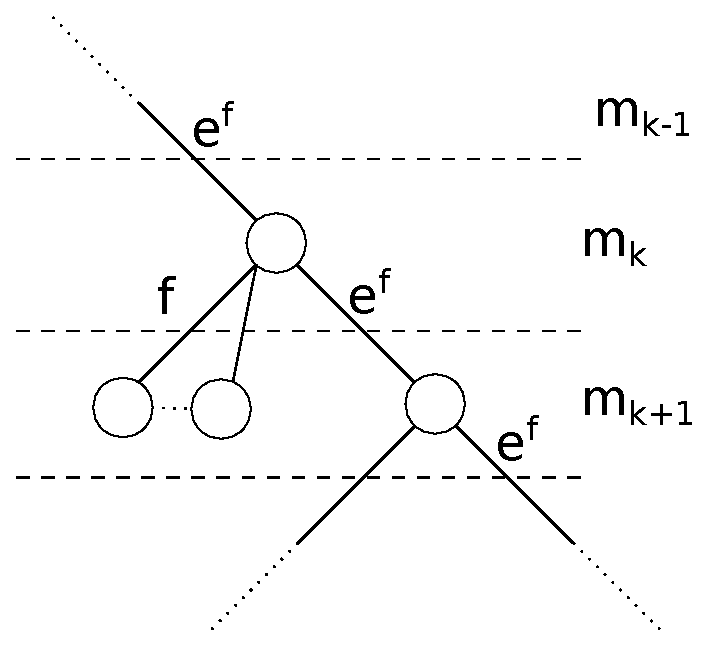
\includegraphics[width = 0.5\textwidth]{./Images/deriv_graph.eps}
	\caption{Illustration of the differentiation scheme.}
	\label{fig:deriv_graph}
\end{figure}

The tree starts with $e^{f(J)}$ at the very top. From there, the derivatives produce a series of terms, one with derivatives of $e^{f(J)}$ and the rest with derivatives of the already present derivatives of $f$. The former is represented by nodes to the right and the latter by nodes to the right. Moving down the tree corresponds to starting with some term, represented by a node, and following the term generated by differentiating a particular factor in that term. For example, there are no factors in front of $e^{f(J)}$ in the beginning, so the tree starts only with a step to the right. In figure \ref{fig:deriv_graph} we see a path that has thus far only included steps to the right, and therefore contains $k - 1$ factors of derivatives of $f$, as well as $e^{f}$. We therefore have $k - 1$ left nodes corresponding to terms with derivatives of these factors, as well as a right node corresponding to the term which has an extra derivative of $f$.

Now, to see the effect of steps in this graph we can perform it explicitly for a sequence of two steps. Supposing we differentiate with respect to $J_{m_{1}}$ and $J_{m_{2}}$, with the $m_{i}$ being some indices, we have
\begin{align*}
	\fdv{J_{m_{2}}}\fdv{J_{m_{1}}}Z[J] &= \fdv{J_{m_{2}}}\left(e^{f(J)}\fdv{f}{J_{m_{1}}}\right) \\
	                                   &= e^{f(J)}\fdv{J_{m_{2}}}\fdv{J_{m_{1}}}f + e^{f(J)}\fdv{f}{J_{m_{2}}}\fdv{f}{J_{m_{1}}}.
\end{align*}
We see that the expression in the bracket in the first line corresponds to there only being a step to the right at the top. From there a derivative of $f$ is produced, so there is exactly one step available to the left and one to the right. These are represented by the left and right terms in the second row.

Three things are now noteworthy with the expression we have arrived at. Firstly, note that the combination of one step left and then one right leaves us with a factor with a second-order derivative of $f$. According to our assumptions, higher-order derivatives of this factor are identically zero, meaning the possibility of a subsequent left step is not present. In other words, each left step corresponds to children nodes having one less left step available than its parent. Next, note both that the term produced from the double right step has two left steps available, one for each factor, confirming a previous claim. Finally, if this were to be the full sequence of derivatives to be computed before setting $J = 0$, only the left term will net a contribution. This is not a coincidence, and in fact it must be that the only nodes at the end of the graph that produce a contribution are those that are reached with an equal amount of right and left steps. This is also very useful, as it indicates directly to us which terms we need to consider.

What is produced from these combinations of left and right steps? To illustrate this, we may add a left step to the term produced by the double right step above. There are two possible left steps from that node, which produces the two terms
\begin{align*}
	e^{f(J)}\fdv{f}{J_{m_{1}}}\fdv{J_{m_{3}}}\fdv{J_{m_{2}}}f + e^{f(J)}\fdv{f}{J_{m_{2}}}\fdv{J_{m_{3}}}\fdv{J_{m_{1}}}f.
\end{align*}
We see that the two right steps produced two first-order derivatives, and the left steps produce the two possible combinations of derivatives with respect to $J_{m_{3}}$ and the other two variables. From this we can infer that the terms that produce non-zero contributions will each contain a set of factors
\begin{align*}
	\fdv{J_{m_{i}}}\fdv{J_{m_{j}}}f
\end{align*}
such that each $m_{i}$ appears exactly once in the full product, and the terms will combine such that all possible pairings of $m_{i}$ and $m_{j}$ are found. For example, in the case of a fourth-order derivative there will be three terms, generated by the pairings according to
\begin{align*}
	&(1, 2), (3, 4) \to \left(\fdv{J_{m_{1}}}\fdv{J_{m_{2}}}f\right)\left(\fdv{J_{m_{3}}}\fdv{J_{m_{4}}}f\right), \\
	&(1, 3), (4, 2) \to \left(\fdv{J_{m_{1}}}\fdv{J_{m_{3}}}f\right)\left(\fdv{J_{m_{4}}}\fdv{J_{m_{2}}}f\right), \\
	&(1, 4), (2, 3) \to \left(\fdv{J_{m_{1}}}\fdv{J_{m_{4}}}f\right)\left(\fdv{J_{m_{2}}}\fdv{J_{m_{3}}}f\right).
\end{align*}
This completes the proof, and what remains to be specified is the values that the second-order functional derivatives take. The final value will also be scaled by the constant $C$.

\paragraph{The Generating Functional for a Free Scalar Field}
Consider the non-interacting scalar field theory with Lagrangian
\begin{align*}
	\lag = -\frac{1}{2}\del{}{\mu}\phi\del{\mu}{}\phi - \frac{1}{2}m^{2}\phi^{2},
\end{align*}
taken with the field to approach zero at infinity. Before writing the generating functional, we rewrite the action as
\begin{align*}
	S &= \integ[4]{}{}{x}{-\frac{1}{2}\del{}{\mu}\phi\del{\mu}{}\phi - \frac{1}{2}m^{2}\phi^{2}} \\
	  &= \integ[4]{}{}{x}{-\frac{1}{2}\left(\del{}{\mu}\left(\phi\del{\mu}{}\phi\right) - \phi\del{}{\mu}\del{\mu}{}\phi\right) - \frac{1}{2}m^{2}\phi^{2}} \\
	  &= \integ[4]{}{}{x}{-\frac{1}{2}\phi\dalem\phi - \frac{1}{2}m^{2}\phi^{2}} \\
	  &= \integ[4]{}{}{x}{\frac{1}{2}\phi\left(-\dalem - m^{2}\right)\phi},
\end{align*}
where we have introduced the d'Alembert operator $-\del{}{\mu}\del{\mu}{}$. Next we are going to use a clever trick by introducing the Klein-Gordon propagator $i\tilde{G} = \Delta$, which satisfies
\begin{align*}
	\left(-\dalem - m^{2}\right)\tilde{G} = \delta^{4}(x - y).
\end{align*}
We then have
\begin{align*}
	\integ[4]{}{}{x}{-\frac{1}{2}\del{}{\mu}\phi\del{\mu}{}\phi - \frac{1}{2}m^{2}\phi^{2} + \phi J} &= \integ[4]{}{}{x}{\frac{1}{2}\phi\left(-\dalem - m^{2}\right)\phi + \phi\integ[4]{}{}{y}{\delta^{4}(x - y)J(y)}} \\
	&= \integ[4]{}{}{x}{\frac{1}{2}\phi\left(-\dalem_{x} - m^{2}\right)\phi + \phi\integ[4]{}{}{y}{J(y)\left(-\dalem_{x} - m^{2}\right)\tilde{G}(x, y)}}.
\end{align*}
We could do some very neat completing of squares here, but that would require
\begin{align*}
	\integ[4]{}{}{y}{J(y)\tilde{G}(x, y)\left(-\dalem_{x} - m^{2}\right)\phi} = \phi(x)J(x).
\end{align*}
To prove that we will perform some clever integration by parts. We have
\begin{align*}
	-\integ[4]{}{}{y}{J(y)\tilde{G}(x, y)\dalem_{x}\phi} &= \integ[4]{}{}{y}{\del{}{\mu}\left(J(y)\tilde{G}(x, y)\del{\mu}{}\phi\right) - J(y)\del{}{\mu}\tilde{G}(x, y)\del{\mu}{}\phi} \\
	&= -\integ[4]{}{}{y}{\del{\mu}{}(J(y)\del{}{\mu}\tilde{G}(x, y)\phi) + J(y)\phi\dalem_{x}\tilde{G}(x, y)} \\
	&= -\integ[4]{}{}{y}{J(y)\phi\dalem_{x}\tilde{G}(x, y)}.
\end{align*}
This completes the proof, and we thus have
\begin{align*}
	\integ[4]{}{}{x}{-\frac{1}{2}\del{}{\mu}\phi\del{\mu}{}\phi - \frac{1}{2}m^{2}\phi^{2} + \phi J} =& \integ[4]{}{}{x}{\frac{1}{2}\phi\left(-\dalem_{x} - m^{2}\right)\phi \\
	&+ \frac{1}{2}\left(\integ[4]{}{}{y}{\phi(x)J(y)\left(-\dalem_{x} - m^{2}\right)\tilde{G}(x, y) + J(y)\tilde{G}(x, y)}\left(-\dalem_{x} - m^{2}\right)\phi(x)\right)} \\
	=& \frac{1}{2}\integ[4]{}{}{x}{\left(\phi + \integ[4]{}{}{y}{J(y)G(x, y)}\right)\left(-\dalem_{x} - m^{2}\right)\left(\phi + \integ[4]{}{}{z}{J(z)G(x, z)}\right) \\
	 &- \integ[4]{}{}{y}{\integ[4]{}{}{z}{J(y)G(x, y)\left(-\dalem_{x} - m^{2}\right)J(z)G(x, z)}}}.
\end{align*}
The final integral can be simplified as
\begin{align*}
	\integ[4]{}{}{x}{\integ[4]{}{}{y}{\integ[4]{}{}{z}{J(y)G(x, y)\left(-\dalem_{x} - m^{2}\right)J(z)G(x, z)}}} &= \integ[4]{}{}{x}{\integ[4]{}{}{y}{\integ[4]{}{}{z}{J(y)G(x, y)J(z)\delta^{4}(x - z)}}} \\
	                           &= \integ[4]{}{}{x}{\integ[4]{}{}{y}{J(y)G(x, y)J(x)}}.
\end{align*}
Now define a new field
\begin{align*}
	\chi(x) = \phi(x) + \integ[4]{}{}{y}{J(y)G(x, y)}.
\end{align*}
This shift has no effect on the integration measure in the path integral, hence we have
\begin{align*}
	Z &= \pinte{}{\chi}e^{\frac{i}{2}\integ[4]{}{}{x}{\chi(x)\left(-\dalem_{x} - m^{2}\right)\chi(y) - \integ[4]{}{}{y}{J(y)G(x, y)J(x)}}} \\
	  &= Ne^{-\frac{1}{2}\integ[4]{}{}{x}{\integ[4]{}{}{y}{J(y)\Delta(x, y)J(x)}}}.
\end{align*}

Let's do a sanity check now, to be sure. We have
\begin{align*}
	&G(x_{1}, x_{2}) = \frac{1}{Z(0)}\left(-i\fdv{J(x_{1})}\right)\left(-i\fdv{J(x_{2})}\right)N_{c}e^{-\frac{1}{2}\integ[4]{}{}{x}{\integ[4]{}{}{y}{J(y)\Delta(x, y)J(x)}}} \\
	                =& \fdv{J(x_{1})}\left(\frac{1}{2}\integ[4]{}{}{x}{\integ[4]{}{}{y}{J(y)\Delta(x, y)\delta^{4}(x - x_{2})}} + \frac{1}{2}\integ[4]{}{}{x}{\integ[4]{}{}{y}{\delta^{4}(y - x_{2})\Delta(x, y)J(x)}}\right)e^{-\frac{1}{2}\integ[4]{}{}{x}{\integ[4]{}{}{y}{J(y)\Delta(x, y)J(x)}}} \\
	                =& \fdv{J(x_{1})}\left(\frac{1}{2}\integ[4]{}{}{y}{J(y)\Delta(x_{2}, y)} + \frac{1}{2}\integ[4]{}{}{x}{\Delta(x, x_{2})J(x)}\right)e^{-\frac{1}{2}\integ[4]{}{}{x}{\integ[4]{}{}{y}{J(y)\Delta(x, y)J(x)}}}.
\end{align*}
We would in principle need to apply the product rule, but it is now obvious that only the term which applies the functional derivative to the non-exponential part will give a non-zero contribution, hence we find
\begin{align*}
	G(x_{1}, x_{2}) = \frac{1}{2}(\Delta(x_{1}, x_{2}) + \Delta(x_{2}, x_{1})),
\end{align*}
and using the fact that the propagator is symmetric under switching the two arguments we have
\begin{align*}
	G(x_{1}, x_{2}) = \Delta(x_{1}, x_{2}),
\end{align*}
as expected.

As a side note, the Feynman diagram for this process is shown in figure \ref{fig:free_scalar_fd}.
\begin{figure}[!ht]
	\centering
	\begin{tikzpicture}
		\begin{feynman}
			\vertex (a1) at (0, 0) {$x_{1}$};
			\vertex (a2) at (3, 0) {$x_{2}$};
			\diagram*{
				(a1) --[scalar] (a2),
			};
		\end{feynman}
	\end{tikzpicture}
	\caption{Feynman diagram for the two-point correlation function for a free scalar.}
	\label{fig:free_scalar_fd}
\end{figure}

\paragraph{The Generating Functional for an Interacting Scalar Field}
Consider the interacting scalar field theory described by
\begin{align*}
	\lag = -\frac{1}{2}\del{}{\mu}\phi\del{\mu}{}\phi - \frac{1}{2}m^{2}\phi^{2} - \frac{1}{4!}\lambda\phi^{4}.
\end{align*}
The generating functional is given by
\begin{align*}
	Z = \pinte{}{\phi}e^{i\left(S_{\text{free}} + \integ[4]{}{}{x}{\phi J - \frac{1}{4!}\lambda\phi^{4}}\right)}.
\end{align*}
We will be working in the framework of perturbation theory and will therefore at some point take the parameter $\lambda$ to be small. We prepare for that by performing a series expansion in $\lambda$ according to
\begin{align*}
	Z = \sum\limits_{m = 0}^{\infty}\frac{1}{m!}\left(-\frac{i\lambda}{4!}\right)^{m}\pinte{}{\phi}\left(\integ[4]{}{}{x}{\phi^{4}}\right)^{m}e^{i\left(S_{\text{free}} + \integ[4]{}{}{x}{\phi J}\right)}.
\end{align*}
Here comes the kicker: The fields can be brought down from the exponent by functional differentiation. Now, that differentiation has no dependence on $\phi$, hence we may extract it from the path integral to find
\begin{align*}
	Z &= \sum\limits_{m = 0}^{\infty}\frac{1}{m!}\left(-\frac{i\lambda}{4!}\right)^{m}\left(\integ[4]{}{}{x}{\left(-i\fdv{J(x)}\right)^{4}}\right)^{m}\pinte{}{\phi}e^{i\left(S_{\text{free}} + \integ[4]{}{}{x}{\phi J}\right)} \\
	  &= \sum\limits_{m = 0}^{\infty}\frac{1}{m!}\left(-\frac{i\lambda}{4!}\right)^{m}\left(\integ[4]{}{}{x}{\left(-i\fdv{J(x)}\right)^{4}}\right)^{m}Z_{\text{free}}.
\end{align*}
This can be related to Feynman diagrams in a very straightforward way.
%TODO: Complete

\paragraph{The Generating Functional in Momentum Space}
Introducing the Fourier transform
\begin{align*}
	\phi(x) = \inte{}{}\frac{\dd[4]{k}}{(2\pi)^{4}}\tilde{\phi}(k)e^{ikx},
\end{align*}
we can write the $n$-point correlation function as
\begin{align*}
	G(x_{1}, \dots, x_{n}) = \frac{1}{Z(0)}\pinte{}{\phi}e^{iS}\inte{}{}\frac{\dd[4]{k_{1}}}{(2\pi)^{4}}\dots \frac{\dd[4]{k_{n}}}{(2\pi)^{4}}e^{i\sum\limits_{i}k_{i}x_{i}}\tilde{\phi}(k_{1})\dots \tilde{\phi}(k_{n}).
\end{align*}
Defining
\begin{align*}
	G(x_{1}, \dots, x_{n}) = \inte{}{}\frac{\dd[4]{k_{1}}}{(2\pi)^{4}}\dots \frac{\dd[4]{k_{n}}}{(2\pi)^{4}}e^{i\sum\limits_{i}k_{i}x_{i}}\tilde{G}(k_{1}, \dots, k_{n})
\end{align*}
we then see
\begin{align*}
	\tilde{G}(k_{1}, \dots, k_{n}) = \frac{1}{Z(0)}\pinte{}{\phi}e^{iS}\tilde{\phi}(k_{1})\dots \tilde{\phi}(k_{n}).
\end{align*}
To write this even more neatly we note that we could in principle switch the path integral to be over $\tilde{\phi}$. This will at most produce a dimensional factor which is equal in the numerator and denominator, provided that we can appropriately define the generating functional. Let us therefore do this.

Consider the integral
\begin{align*}
	\inte{}{}\dd[4]{x}\phi(x)J(x) &= \inte{}{}\dd[4]{x}\inte{}{}\frac{\dd[4]{k_{1}}}{(2\pi)^{4}}\frac{\dd[4]{k_{2}}}{(2\pi)^{4}}e^{i(k_{1}x + k_{2}x)}\tilde{\phi}(k_{1})\tilde{J}(k_{2}).
\end{align*}
The two integrals arise because we are considering two different functions with their own unique Fourier transforms. Performing the $x$ integration we find
\begin{align*}
	\inte{}{}\dd[4]{x}\inte{}{}\frac{\dd[4]{k_{1}}}{(2\pi)^{4}}\frac{\dd[4]{k_{2}}}{(2\pi)^{4}}e^{i(k_{1}x + k_{2}x)}\tilde{\phi}(k_{1})\tilde{J}(k_{2}) &= \inte{}{}\frac{\dd[4]{k_{1}}\dd[4]{k_{2}}}{(2\pi)^{4}}\delta^{4}(k_{1} + k_{2})\tilde{\phi}(k_{1})\tilde{J}(k_{2}) \\
	&= \inte{}{}\frac{\dd[4]{k}}{(2\pi)^{4}}\tilde{\phi}(k)\tilde{J}(-k).
\end{align*}
Note the structure of this result, as it will be reused regularly. Pending a rewrite of the action in terms of $\tilde{\phi}$ we have
\begin{align*}
	Z[J] &= \pinte{}{\phi}e^{i\left(S[\phi] + \inte{}{}\dd[4]{x}\phi J\right)} \\
	     &= \pinte{}{\phi}e^{i\left(S[\tilde{\phi}] + \inte{}{}\frac{\dd[4]{k}}{(2\pi)^{4}}\tilde{\phi}(k)\tilde{J}(-k)\right)}.
\end{align*}
The change of integration measure involves a dimensional factor, as previously stated, but because it will always be common for factors in a numerator and denominator, we may define
\begin{align*}
	Z[\tilde{J}] &= \pinte{}{\tilde{\phi}}e^{i\left(S[\tilde{\phi}] + \inte{}{}\frac{\dd[4]{k}}{(2\pi)^{4}}\tilde{\phi}(k)\tilde{J}(-k)\right)}.
\end{align*}
This functional evidently satisfies
\begin{align*}
	\tilde{G}(k_{1}, \dots, k_{n}) = \frac{1}{Z[0]}\eval{\left(-i(2\pi)^{4}\fdv{\tilde{J}(-k_{1})}\right)\dots\left(-i(2\pi)^{4}\fdv{\tilde{J}(-k_{n})}\right)Z[\tilde{J}]}_{\tilde{J} = 0}.
\end{align*}
%TODO: Propagate correction

\paragraph{Momentum Space Generating Functional for a Free Scalar}
We once again consider a system with Lagrangian
\begin{align*}
	\lag = -\frac{1}{2}\del{}{\mu}\phi\del{\mu}{}\phi - \frac{1}{2}m^{2}\phi^{2}.
\end{align*}
The action can then be written as
\begin{align*}
	S &= \integ[4]{}{}{x}{-\frac{1}{2}\del{}{\mu}\phi\del{\mu}{}\phi - \frac{1}{2}m^{2}\phi^{2}} \\
	  &= \integ[4]{}{}{x}{\frac{1}{2}\phi\left(-\dalem - m^{2}\right)\phi} \\
	  &= \frac{1}{2}\integ[4]{}{}{x}{\inte{}{}\frac{\dd[4]{k_{1}}}{(2\pi)^{4}}\frac{\dd[4]{k_{2}}}{(2\pi)^{4}}e^{ik_{1}x}\tilde{\phi}(k_{1})\left(-\dalem - m^{2}\right)\left(e^{ik_{2}x}\tilde{\phi}(k_{2})\right)} \\
	  &= \frac{1}{2}\integ[4]{}{}{x}{\inte{}{}\frac{\dd[4]{k_{1}}}{(2\pi)^{4}}\frac{\dd[4]{k_{2}}}{(2\pi)^{4}}e^{ik_{1}x}\tilde{\phi}(k_{1})\left(-k_{2}^{2} - m^{2}\right)e^{ik_{2}x}\tilde{\phi}(k_{2})} \\
	  &= -\frac{1}{2}\inte{}{}\frac{\dd[4]{k}}{(2\pi)^{4}}\tilde{\phi}(-k)\left(k^{2} + m^{2}\right)\tilde{\phi}(k).
\end{align*}
The integral in the exponent can once again, this time with a very straight-forward ompleting of the square, be written as
\begin{align*}
	 &\inte{}{}\frac{\dd[4]{k}}{(2\pi)^{4}}-\frac{1}{2}\tilde{\phi}(-k)\left(k^{2} + m^{2}\right)\tilde{\phi}(k) + \tilde{\phi}(k)\tilde{J}(-k) \\
	=& \inte{}{}\frac{\dd[4]{k}}{(2\pi)^{4}}-\frac{1}{2}\tilde{\phi}(-k)\left(k^{2} + m^{2}\right)\tilde{\phi}(k) + \frac{1}{2}(\tilde{\phi}(k)\tilde{J}(-k) + \tilde{\phi}(-k)\tilde{J}(k)) \\
	=& -\frac{1}{2}\inte{}{}\frac{\dd[4]{k}}{(2\pi)^{4}}\left(\tilde{\phi}(-k) - \frac{1}{k^{2} + m^{2}}\tilde{J}(-k)\right)\left(k^{2} + m^{2}\right)\left(\tilde{\phi}(k) - \frac{1}{k^{2} + m^{2}}\tilde{J}(k)\right) - \frac{1}{k^{2} + m^{2}}\tilde{J}(k)\tilde{J}(-k).
\end{align*}
Defining
\begin{align*}
	\tilde{\chi} = \tilde{\phi}(k) - \frac{1}{k^{2} + m^{2}}\tilde{J}(k)
\end{align*}
and switching the integration measure we find
\begin{align*}
	\gf{\tilde{J}} &= Ne^{\frac{i}{2}\inte{}{}\frac{\dd[4]{k}}{(2\pi)^{4}}\frac{1}{k^{2} + m^{2}}\tilde{J}(k)\tilde{J}(-k)}.
\end{align*}

Let us once again perform a sanity check. We have
\begin{align*}
	\tilde{G}(k_{1}, k_{2}) &= \eval{-(2\pi)^{8}\fdv{\tilde{J}(k_{1})}\frac{i}{2(2\pi)^{4}}\left(\frac{1}{k_{2}^{2} + m^{2}}\tilde{J}(-k_{2}) + \frac{1}{k_{2}^{2} + m^{2}}\tilde{J}(-k_{2})\right)e^{\frac{i}{2}\inte{}{}\frac{\dd[4]{k}}{(2\pi)^{4}}\frac{1}{k^{2} + m^{2}}\tilde{J}(k)\tilde{J}(-k)}}_{\tilde{J} = 0} \\
	&= \eval{-i(2\pi)^{4}\fdv{\tilde{J}(k_{1})}\frac{1}{k_{2}^{2} + m^{2}}\tilde{J}(-k_{2})e^{\frac{i}{2}\inte{}{}\frac{\dd[4]{k}}{(2\pi)^{4}}\frac{1}{k^{2} + m^{2}}\tilde{J}(k)\tilde{J}(-k)}}_{\tilde{J} = 0}.
\end{align*}
Once again the contribution from the second differentiation of the exponential can be ignored and we find
\begin{align*}
	\tilde{G}(k_{1}, k_{2}) &= -i(2\pi)^{4}\frac{1}{k_{2}^{2} + m^{2}}\delta^{4}(k_{1} + k_{2}).
\end{align*}
This is very similar to the momentum-space propagator, except that it only implicitly contains information about $G$ only being a function of the displacement between two points.

\paragraph{Momentum Space Generating Functional for an Interacting Scalar}
We now consider an interacting scalar field with Lagrangian
\begin{align*}
	\lag = -\frac{1}{2}\del{}{\mu}\phi\del{\mu}{}\phi - \frac{1}{2}m^{2}\phi^{2} - \frac{1}{4!}\lambda\phi^{4}.
\end{align*}
The interacting part of the action can be rewritten as
\begin{align*}
	S &= -\frac{1}{4!}\lambda\integ[4]{}{}{x}{\inte{}{}\frac{\dd[4]{k_{1}}}{(2\pi)^{4}}\frac{\dd[4]{k_{2}}}{(2\pi)^{4}}\frac{\dd[4]{k_{3}}}{(2\pi)^{4}}\frac{\dd[4]{k_{4}}}{(2\pi)^{4}}\tilde{\phi}(k_{1})\tilde{\phi}(k_{2})\tilde{\phi}(k_{3})\tilde{\phi}(k_{4})e^{ix\sum\limits_{i}k_{i}}} \\
	  &= -\frac{1}{4!}\lambda\inte{}{}\frac{\dd[4]{k_{1}}}{(2\pi)^{4}}\frac{\dd[4]{k_{2}}}{(2\pi)^{4}}\frac{\dd[4]{k_{3}}}{(2\pi)^{4}}\frac{\dd[4]{k_{4}}}{(2\pi)^{4}}\delta^{4}\left(\sum\limits_{i}k_{i}\right)\tilde{\phi}(k_{1})\tilde{\phi}(k_{2})\tilde{\phi}(k_{3})\tilde{\phi}(k_{4}).
\end{align*}
Similar to the position space case we then have
\begin{align*}
	&Z[\tilde{J}] \\
   =& \pinte{}{\phi}e^{i\left(-\inte{}{}\frac{\dd[4]{k}}{(2\pi)^{4}}\frac{1}{2}\tilde{\phi}(k)\left(-k^{2} + m^{2}\right)\tilde{\phi}(-k) - \frac{\lambda}{4!}\inte{}{}\frac{\dd[4]{k}_{1}}{(2\pi)^{4}}\frac{\dd[4]{k}_{2}}{(2\pi)^{4}}\frac{\dd[4]{k}_{3}}{(2\pi)^{4}}\frac{\dd[4]{k}_{4}}{(2\pi)^{4}}\delta^{4}\left(\sum\limits_{i = 1}^{4}k_{i}\right)\tilde{\phi}(k_{1})\tilde{\phi}(k_{2})\tilde{\phi}(k_{3})\tilde{\phi}(k_{4}) + \inte{}{}\frac{\dd[4]{k}}{(2\pi)^{4}}\tilde{\phi}(k)\tilde{J}(-k)\right)} \\
   =& \sum\limits_{m = 0}^{\infty}\frac{1}{m!}\left(-\frac{i\lambda}{4!}\right)^{m} \\
    &\cdot\pinte{}{\tilde{\phi}}\left(\inte{}{}\left(\prod\limits_{j = 1}^{4}\frac{\dd[4]{k_{i}}}{(2\pi)^{4}}\right)\delta^{4}\left(\sum\limits_{i}k_{i}\right)\tilde{\phi}(k_{1})\tilde{\phi}(k_{2})\tilde{\phi}(k_{3})\tilde{\phi}(k_{4})\right)^{m}e^{i\left(S_{\text{free}} + \inte{}{}\frac{\dd[4]{k}}{(2\pi)^{4}}\tilde{\phi}(k)\tilde{J}(-k)\right)} \\
   =& \sum\limits_{m = 0}^{\infty}\frac{1}{m!}\left(-\frac{i\lambda}{4!}\right)^{m} \\
    &\cdot\pinte{}{\tilde{\phi}}\left(\inte{}{}\left(\prod\limits_{j = 1}^{4}\frac{\dd[4]{k_{i}}}{(2\pi)^{4}}\right)\delta^{4}\left(\sum\limits_{i}k_{i}\right)(-(2\pi)^{4}i)^{4}\fdv{\tilde{J}(k_{1})}\fdv{\tilde{J}(k_{2})}\fdv{\tilde{J}(k_{3})}\fdv{\tilde{J}(k_{4})}\right)^{m}e^{i\left(S_{\text{free}} + \inte{}{}\frac{\dd[4]{k}}{(2\pi)^{4}}\tilde{\phi}(k)\tilde{J}(-k)\right)} \\
   =& \sum\limits_{m = 0}^{\infty}\frac{1}{m!}\left(-\frac{i\lambda}{4!}\right)^{m} \\
    &\cdot\left(\inte{}{}\left(\prod\limits_{j = 1}^{4}\frac{\dd[4]{k_{i}}}{(2\pi)^{4}}\right)\delta^{4}\left(\sum\limits_{i}k_{i}\right)(-(2\pi)^{4}i)^{4}\fdv{\tilde{J}(k_{1})}\fdv{\tilde{J}(k_{2})}\fdv{\tilde{J}(k_{3})}\fdv{\tilde{J}(k_{4})}\right)^{m}\pinte{}{\tilde{\phi}}e^{i\left(S_{\text{free}} + \inte{}{}\frac{\dd[4]{k}}{(2\pi)^{4}}\tilde{\phi}(k)\tilde{J}(-k)\right)} \\
   =& \sum\limits_{m = 0}^{\infty}\frac{1}{m!}\left(-\frac{i\lambda}{4!}\right)^{m}\left(\inte{}{}\left(\prod\limits_{j = 1}^{4}\frac{\dd[4]{k_{i}}}{(2\pi)^{4}}\right)\delta^{4}\left(\sum\limits_{i}k_{i}\right)(-(2\pi)^{4}i)^{4}\fdv{\tilde{J}(k_{1})}\fdv{\tilde{J}(k_{2})}\fdv{\tilde{J}(k_{3})}\fdv{\tilde{J}(k_{4})}\right)^{m}Z_{\text{free}}[\tilde{J}].
\end{align*}
This can also be used to derive Feynman rules.
%TODO: Complete

Once again we start with the momentum space generating functional
\begin{align*}
Z[\tilde{J}] = Ne^{\frac{i}{2}\inte{}{}\frac{\dd[4]{k}}{(2\pi)^{4}}\frac{1}{k^{2} + m^{2} + i\epsilon}\tilde{J}(k)\tilde{J}(-k)},
\end{align*}
which was derived in class. We can now series expand the generating functional for the interacting case according to
\begin{align*}
&Z[\tilde{J}] \\
=& \pinte{}{\phi}e^{i\left(-\inte{}{}\frac{\dd[4]{k}}{(2\pi)^{4}}\frac{1}{2}\tilde{\phi}(k)\left(-k^{2} + m^{2}\right)\tilde{\phi}(-k) - \frac{\lambda}{4!}\inte{}{}\frac{\dd[4]{k}_{1}}{(2\pi)^{4}}\frac{\dd[4]{k}_{2}}{(2\pi)^{4}}\frac{\dd[4]{k}_{3}}{(2\pi)^{4}}\frac{\dd[4]{k}_{4}}{(2\pi)^{4}}\delta^{4}\left(\sum\limits_{i = 1}^{4}k_{i}\right)\tilde{\phi}(k_{1})\tilde{\phi}(k_{2})\tilde{\phi}(k_{3})\tilde{\phi}(k_{4}) + \inte{}{}\frac{\dd[4]{k}}{(2\pi)^{4}}\tilde{\phi}(k)\tilde{J}(-k)\right)} \\
=& \sum\limits_{m = 0}^{\infty}\frac{1}{m!}\left(-\frac{i\lambda}{4!}\right)^{m} \\
&\cdot\pinte{}{\tilde{\phi}}\left(\inte{}{}\left(\prod\limits_{j = 1}^{4}\frac{\dd[4]{k_{i}}}{(2\pi)^{4}}\right)\delta^{4}\left(\sum\limits_{i}k_{i}\right)\tilde{\phi}(k_{1})\tilde{\phi}(k_{2})\tilde{\phi}(k_{3})\tilde{\phi}(k_{4})\right)^{m}e^{i\left(S_{\text{free}} + \inte{}{}\frac{\dd[4]{k}}{(2\pi)^{4}}\tilde{\phi}(k)\tilde{J}(-k)\right)} \\
=& \sum\limits_{m = 0}^{\infty}\frac{1}{m!}\left(-\frac{i\lambda}{4!}\right)^{m} \\
&\cdot\pinte{}{\tilde{\phi}}\left(\inte{}{}\left(\prod\limits_{j = 1}^{4}\frac{\dd[4]{k_{i}}}{(2\pi)^{4}}\right)\delta^{4}\left(\sum\limits_{i}k_{i}\right)(-(2\pi)^{4}i)^{4}\fdv{\tilde{J}(k_{1})}\fdv{\tilde{J}(k_{2})}\fdv{\tilde{J}(k_{3})}\fdv{\tilde{J}(k_{4})}\right)^{m}e^{i\left(S_{\text{free}} + \inte{}{}\frac{\dd[4]{k}}{(2\pi)^{4}}\tilde{\phi}(k)\tilde{J}(-k)\right)} \\
=& \sum\limits_{m = 0}^{\infty}\frac{1}{m!}\left(-\frac{i\lambda}{4!}\right)^{m} \\
&\cdot\left(\inte{}{}\left(\prod\limits_{j = 1}^{4}\frac{\dd[4]{k_{i}}}{(2\pi)^{4}}\right)\delta^{4}\left(\sum\limits_{i}k_{i}\right)(-(2\pi)^{4}i)^{4}\fdv{\tilde{J}(k_{1})}\fdv{\tilde{J}(k_{2})}\fdv{\tilde{J}(k_{3})}\fdv{\tilde{J}(k_{4})}\right)^{m}\pinte{}{\tilde{\phi}}e^{i\left(S_{\text{free}} + \inte{}{}\frac{\dd[4]{k}}{(2\pi)^{4}}\tilde{\phi}(k)\tilde{J}(-k)\right)} \\
=& \sum\limits_{m = 0}^{\infty}\frac{1}{m!}\left(-\frac{i\lambda}{4!}\right)^{m}\left(\inte{}{}\left(\prod\limits_{j = 1}^{4}\frac{\dd[4]{k_{i}}}{(2\pi)^{4}}\right)\delta^{4}\left(\sum\limits_{i}k_{i}\right)(-(2\pi)^{4}i)^{4}\fdv{\tilde{J}(k_{1})}\fdv{\tilde{J}(k_{2})}\fdv{\tilde{J}(k_{3})}\fdv{\tilde{J}(k_{4})}\right)^{m}Z_{\text{free}}[\tilde{J}].
\end{align*}

The functional derivatives can be handled using Wick's theorem, provided we compute the second-order functional derivatives. We have
\begin{align*}
&(2\pi)^{8}(-i)^{2}\fdv{\tilde{J}(k_{1})}\fdv{\tilde{J}(k_{2})}Z_{\text{free}} \\
=& -i(2\pi)^{8}\fdv{\tilde{J}(k_{1})}\frac{N}{2}\left(\inte{}{}\frac{\dd[4]{k}}{(2\pi)^{4}}\frac{1}{k^{2} + m^{2} + i\epsilon}\left(\delta^{4}(k - k_{2})\tilde{J}(-k) + J(k)\delta^{4}(k + k_{2})\right)\right)e^{\frac{i}{2}\inte{}{}\frac{\dd[4]{k}}{(2\pi)^{4}}\frac{1}{k^{2} + m^{2} + i\epsilon}\tilde{J}(k)\tilde{J}(-k)} \\
=& -i(2\pi)^{4}\frac{N}{2}\fdv{\tilde{J}(k_{1})}\frac{1}{k_{2}^{2} + m^{2} + i\epsilon}\left(\tilde{J}(-k_{2}) + J(-k_{2})\right)e^{\frac{i}{2}\inte{}{}\frac{\dd[4]{k}}{(2\pi)^{4}}\frac{1}{k^{2} + m^{2} + i\epsilon}\tilde{J}(k)\tilde{J}(-k)} \\
=& -i(2\pi)^{4}\frac{N}{2}\left(\frac{2}{k_{2}^{2} + m^{2} + i\epsilon}\delta^{4}(k_{1} + k_{2}) + \frac{2}{k_{1}^{2} + m^{2} + i\epsilon}\frac{2i}{k_{2}^{2} + m^{2} + i\epsilon}\tilde{J}(-k_{1})\tilde{J}(-k_{2})\right)e^{\frac{i}{2}\inte{}{}\frac{\dd[4]{k}}{(2\pi)^{4}}\frac{1}{k^{2} + m^{2} + i\epsilon}\tilde{J}(k)\tilde{J}(-k)},
\end{align*}
and evaluation at $\tilde{J} = 0$ yields the result
\begin{align*}
\eval{(2\pi)^{8}(-i)^{2}\fdv{\tilde{J}(k_{1})}\fdv{\tilde{J}(k_{2})}Z_{\text{free}}}_{\tilde{J} = 0} = -i(2\pi)^{4}N\frac{1}{k_{2}^{2} + m^{2} + i\epsilon}\delta^{4}(k_{1} + k_{2}).
\end{align*}
We write this as
\begin{align*}
\eval{(2\pi)^{8}(-i)^{2}\fdv{\tilde{J}(k_{1})}\fdv{\tilde{J}(k_{2})}Z_{\text{free}}}_{\tilde{J} = 0} = N\Delta(k_{1}, k_{2}).
\end{align*}

In order to compute the $4$-point correlation function to order $2$ in $\lambda$ we will first need the generating functional itself to order $2$. The zeroth-order term is trivial. Using Wick's theorem, the first-order term is
\begin{align*}
-\frac{iN\lambda}{4!}\inte{}{}\left(\prod\limits_{j = 1}^{4}\frac{\dd[4]{k_{i}}}{(2\pi)^{4}}\right)\delta^{4}\left(\sum\limits_{i}k_{i}\right)\left(\Delta(k_{1}, k_{2})\Delta(k_{3}, k_{4}) + \Delta(k_{1}, k_{3})\Delta(k_{4}, k_{2}) + \Delta(k_{1}, k_{4})\Delta(k_{2}, k_{3})\right).
\end{align*}
Of course these are all identical, as there is no significance in the labelling of the momenta. Hence the first-order term is
\begin{align*}
-3\frac{iN\lambda}{4!}\inte{}{}\left(\prod\limits_{j = 1}^{4}\frac{\dd[4]{k_{i}}}{(2\pi)^{4}}\right)\delta^{4}\left(\sum\limits_{i}k_{i}\right)\Delta(k_{1}, k_{2})\Delta(k_{3}, k_{4}).
\end{align*}
Diagrammatically this is represented in figure \ref{fig:first_order_bubble_fd}.

\begin{figure}[!ht]
	\centering
	\begin{tikzpicture}
	\begin{feynman}
	\vertex (a) at (0, 0);
	\vertex (b) at (-2, 0);
	\vertex (c) at (2, 0);
	\diagram*{
		(a) --[scalar, out = 45, in = 90] (c) --[scalar, out = -90, in = -45] (a),
		(a) --[scalar, out = 135, in = 90] (b) --[scalar, out = -90, in = -135] (a),
	};
	\end{feynman}
	\end{tikzpicture}
	\caption{Feynman diagram for the first-order term in the generating functional.}
	\label{fig:first_order_bubble_fd}
\end{figure}

The second-order term is somewhat more non-trivial due to the Dirac delta function, dividing the momenta into two classes. We can, however, classify the cases in terms of how many momenta are mixed in the arguments of $\Delta$. They are represented by the Feynman diagrams in figure

\begin{figure}[!ht]
	\centering
	\subfloat[No mixing.]{
		\begin{tikzpicture}
		\begin{feynman}
		\vertex (a) at (0, 0);
		\vertex (b) at (-2, 0);
		\vertex (c) at (2, 0);
		\vertex (a1) at (5, 0);
		\vertex (b1) at (3, 0);
		\vertex (c1) at (7, 0);
		\diagram*{
			(a) --[scalar, out = 45, in = 90] (c) --[scalar, out = -90, in = -45] (a),
			(a) --[scalar, out = 135, in = 90] (b) --[scalar, out = -90, in = -135] (a),
			(a1) --[scalar, out = 45, in = 90] (c1) --[scalar, out = -90, in = -45] (a1),
			(a1) --[scalar, out = 135, in = 90] (b1) --[scalar, out = -90, in = -135] (a1),
		};
		\end{feynman}
		\end{tikzpicture}
	} \\
	\subfloat[Two mixed momenta.]{
		\begin{tikzpicture}
		\begin{feynman}
		\vertex (a) at (0, 0);
		\vertex (b) at (-2, 0);
		\vertex (c) at (2, 0);
		\vertex (d) at (4, 0);
		\diagram*{
			(a) --[scalar, out = 45, in = 135] (c) --[scalar, out = 45, in = 90] (d) --[scalar, out = -90, in = -45] (c) --[scalar, out = -135, in = -45] (a),
			(a) --[scalar, out = 135, in = 90] (b) --[scalar, out = -90, in = -135] (a),
		};
		\end{feynman}
		\end{tikzpicture}
	}
	\subfloat[Four mixed momenta.]{
		\begin{tikzpicture}
		\begin{feynman}
		\vertex (a) at (0, 0);
		\vertex (b) at (2, 0);
		\diagram*{
			(a) --[scalar, out = 45, in = 135] (b) --[scalar, out = -135, in = -45] (a),
			(a) --[scalar, half left] (b) --[scalar, half left] (a),
		};
		\end{feynman}
		\end{tikzpicture}
	}
	\caption{Feynman diagrams for the second-order term in the generating functional.}
	\label{fig:first_order_bubble_fd}
\end{figure}

\paragraph{Multiple Scalar Fields}
We now consider a system of multiple scalar fields $\phi^{(a)}$. We take them to be real scalar fields, hence
\begin{align*}
	\left(\tilde{\phi}^{(a)}\right)\cc(k) = \tilde{\phi}^{(a)}(-k).
\end{align*}
The most general action for such a field theory is
\begin{align*}
	S &= \frac{1}{2}\integ[4]{}{}{x}{\phi^{(a)}(x)D_{ab}\phi^{(b)}(x)} = \frac{1}{2}\inte{}{}\frac{\dd[4]{k}}{(2\pi)^{4}}\tilde{\phi}^{(a)}(-k)\tilde{M}_{ab}(k)\tilde{\phi}^{(b)}(k).
\end{align*}
$D$ is a matrix of differential operators and $\tilde{M}$ a matrix of functions. The latter can be symmetrized to
\begin{align*}
	S &= \frac{1}{2}\inte{}{}\frac{\dd[4]{k}}{(2\pi)^{4}}\tilde{\phi}^{(a)}(-k)M_{ab}(k)\tilde{\phi}^{(b)}(k),\ M_{ab}(k) = \frac{1}{2}(\tilde{M}_{ab}(k) + \tilde{M}_{ba}(-k)).
\end{align*}

We can now go about finding a generating functional for this kind of system. We have
\begin{align*}
	Z &= \pinte{}{\phi^{a}}e^{iS + i\integ[4]{}{}{x}{\phi^{(a)}J_{a}}}
\end{align*}
in position space and
\begin{align*}
	Z &= \pinte{}{\tilde{\phi}^{a}}e^{iS + i\inte{}{}\frac{\dd[4]{k}}{(2\pi)^{4}}\tilde{\phi}^{(a)}(k)\tilde{J}_{a}}(-k)
\end{align*}
in momentum space. The latter exponent can be handled the most easily, so we will do that one. We have
\begin{align*}
	S + \inte{}{}\frac{\dd[4]{k}}{(2\pi)^{4}}\tilde{\phi}^{(a)}(k)\tilde{J}_{a}(-k) =& \inte{}{}\frac{\dd[4]{k}}{(2\pi)^{4}}\frac{1}{2}\tilde{\phi}^{(a)}(-k)M_{ab}(k)\tilde{\phi}^{(b)}(k) + \tilde{\phi}^{(a)}(k)\tilde{J}_{a}(-k) \\
	=& \inte{}{}\frac{\dd[4]{k}}{(2\pi)^{4}}\frac{1}{2}\left(\tilde{\phi}^{(a)}(-k) + M_{ac}^{-1}(-k)\tilde{J}_{c}(-k)\right)M_{ab}(k)\left(\tilde{\phi}^{(b)}(k) + M_{bd}^{-1}(k)\tilde{J}_{d}(k)\right) \\
	 &- \inte{}{}\frac{\dd[4]{k}}{(2\pi)^{4}}\frac{1}{2}M_{ac}^{-1}(-k)\tilde{J}_{c}(k)M_{ab}(k)M_{bd}^{-1}(k)\tilde{J}_{d}(k) \\
	=& \inte{}{}\frac{\dd[4]{k}}{(2\pi)^{4}}\frac{1}{2}\tilde{\chi}^{(a)}(-k)M_{ab}(k)\tilde{\chi}^{(b)}(k) - \inte{}{}\frac{\dd[4]{k}}{(2\pi)^{4}}\frac{1}{2}M_{ac}^{-1}(-k)\tilde{J}_{c}(-k)\delta_{ad}\tilde{J}_{d}(k) \\
	=& \frac{1}{2}\inte{}{}\frac{\dd[4]{k}}{(2\pi)^{4}}\tilde{\chi}^{(a)}(-k)M_{ab}(k)\tilde{\chi}^{(b)}(k) - \frac{1}{2}\inte{}{}\frac{\dd[4]{k}}{(2\pi)^{4}}\tilde{J}_{a}(-k)M_{ac}^{-1}(-k)\tilde{J}_{c}(k).
\end{align*}
To do this we have defined the new fields
\begin{align*}
	\tilde{\chi}^{(a)}(k) = \tilde{\phi}^{(a)}(k) + M_{ac}^{-1}(-k)\tilde{J}_{c}(k)
\end{align*}
and used the fact that
\begin{align*}
	M^{-1}(k) = (M^{T}(k))^{-1} = (M^{-1}(k))^{T}.
\end{align*}
This means
\begin{align*}
	Z &= Ne^{-\frac{i}{2}\inte{}{}\frac{\dd[4]{k}}{(2\pi)^{4}}\tilde{J}_{a}(-k)M_{ac}^{-1}(-k)\tilde{J}_{c}(k)}.
\end{align*}
The propagator is then
\begin{align*}
	G_{ab}(k_{1}, k_{2}) =& -(2\pi)^{8}\fdv{\tilde{J}_{a}(k_{1})}\left(-\frac{i}{2}\inte{}{}\frac{\dd[4]{k}}{(2\pi)^{4}}\delta_{bc}\delta^{4}(k + k_{2})M_{cd}^{-1}(-k)\tilde{J}_{d}(k) \right. \\
	&- \left. \frac{i}{2}\inte{}{}\frac{\dd[4]{k}}{(2\pi)^{4}}\tilde{J}_{c}(-k)M_{cd}^{-1}(-k)\delta_{bd}\delta^{4}(k - k_{2})\right)e^{-\frac{i}{2}\inte{}{}\frac{\dd[4]{k}}{(2\pi)^{4}}\tilde{J}_{c}(-k)M_{cd}^{-1}(-k)\tilde{J}_{d}(k)} \\
	=& \frac{(2\pi)^{4}i}{2}\fdv{\tilde{J}_{a}(k_{1})}\left(M_{bd}^{-1}(k_{2})\tilde{J}_{d}(-k_{2}) + \tilde{J}_{c}(-k_{2})M_{cb}^{-1}(-k_{2})\right)e^{-\frac{i}{2}\inte{}{}\frac{\dd[4]{k}}{(2\pi)^{4}}\tilde{J}_{c}(-k)M_{cd}^{-1}(-k)\tilde{J}_{d}(k)} \\
	=& \frac{(2\pi)^{4}i}{2}\left(M_{ba}^{-1}(k_{2}) + M_{ab}^{-1}(-k_{2})\right)\delta^{4}(k_{1} + k_{2}).
\end{align*}

\paragraph{Failing to Quantize the Electromagnetic Field}
The momentum space Lagrangian is
\begin{align*}
	\lag &= -\frac{1}{4}\left(k_{\mu}A_{\nu} - k_{\nu}A_{\mu}\right)\left(k^{\mu}A^{\nu} - k^{\nu}A^{\mu}\right) \\
	     &= -\frac{1}{4}\left(A_{\nu}\left(k^{2}A^{\nu} - k_{\mu}k^{\nu}A^{\mu}\right) - A_{\nu}\left(k_{\mu}k^{\nu}A^{\mu} - k^{2}A^{\nu}\right)\right) \\
	     &= \frac{1}{2}A_{\nu}\left(k^{\mu}k^{\nu}A_{\mu} - k^{2}A^{\nu}\right) \\
	     &= \frac{1}{2}A_{\nu}\left(k^{\mu}k^{\nu} - k^{2}g^{\mu\nu}\right)A_{\mu}.
\end{align*}
This is a bit of a disaster, as $M$ always has at least one eigenvalue of zero. Namely, we have
\begin{align*}
	M^{\mu\nu}k_{\nu} = k^{\mu}k^{\nu}k_{\nu} - k^{2}g^{\mu\nu}k_{\nu} = 0.
\end{align*}
This means that $M^{-1}$ does not exist for any $k$. That scenario is a lot worse than for the Klein-Gordon equation, where $M^{-1}$ only didn't exist at the set of $k$ such that $k^{2} = -m^{2}$.

\paragraph{The Free Dirac Field}
We will quantize Dirac fields by taking
\begin{align*}
	\psi(x) = \sum\limits_{i}\theta_{i}\phi_{i}(x),
\end{align*}
where the $\phi_{i}$ are an appropriate basis of functions and the $\theta_{i}$ are complex Grassman variables. We will pair the fields with the Dirac adjoint rather than the normal adjoint, which is allowed as the two are related by a unitary transform. The action is
\begin{align*}
	S = \integ[4]{}{}{x}{\overline{\psi}_{\alpha}\left(-i\gamma^{\mu}\del{}{\mu} - m\right)_{\alpha\beta}\psi_{\beta}}
\end{align*}
in position space and
\begin{align*}
	S = \inte{}{}\frac{\dd[4]{k}}{(2\pi)^{4}}\tilde{\overline{\psi}}_{\alpha}(-k)\left(\gamma^{\mu}k_{\mu} - m\right)_{\alpha\beta}\tilde{\psi}_{\beta}(k)
\end{align*}
in momentum space. The indices on the fields are Dirac indices. In the generating functional we pair the fields and their adjoints with fields $\tilde{J}$ and $\tilde{\overline{J}}$. According to our definition of derivatives with respect to Grassman variables we then find
\begin{align*}
	\expval{\tilde{\psi}_{\alpha_{1}}(k_{1})\dots\tilde{\psi}_{\alpha_{n}}(k_{n})\tilde{\overline{\psi}}_{\beta_{1}}(p_{1})\dots\tilde{\overline{\psi}}_{\beta_{n}}(p_{n})}{\Omega} = \prod\limits_{i}\left(-i(2\pi)^{4}\fdv{\tilde{\overline{J}}(k_{i})}\right)\prod\limits_{i}\left(i(2\pi)^{4}\fdv{\tilde{J}(p_{i})}\right)Z.
\end{align*}
%TODO: Show
We can show that
\begin{align*}
	Z = Ne^{-i\inte{}{}\frac{\dd[4]{k}}{(2\pi)^{4}}\tilde{\overline{J}}_{\alpha}(-k)(\fsl{k} - m)_{\alpha\beta}^{-1}\tilde{J}_{\beta}(k)},
\end{align*}
and from this recover familiar results.

\paragraph{An Interacting Fermion Theory}
%TODO: Expand
Consider a field theory with a Dirac field, a scalar field and an interaction term
\begin{align*}
	\lag = \lambda\overline{\psi}\psi\phi.
\end{align*}

\paragraph{A Go at Quantum Electrodynamics}
Quantum electrodynamics starts with wanting to extend the global gauge symmetry of the free fermionic field to a local. This is done by replacing the derivative with
\begin{align*}
	D_{\mu} = \del{}{\mu} - ieA_{\mu},
\end{align*}
where $A$ is the so-called gauge field. The full gauge transformation is
\begin{align*}
	\Psi\to e^{i\lambda(x)}\Psi,\ A_{\mu}\to A_{\mu} + \del{}{\mu}\lambda.
\end{align*}
For the field theory to work we now need to add terms describing $A$ to the action, starting with quadratic ones as these are the easiest. The quantity
\begin{align*}
	F_{\mu\nu} = \comm{D_{\mu}}{D_{\nu}}
\end{align*}
is gauge invariant, so we add
\begin{align*}
	\lag = -\frac{1}{4}F_{\mu\nu}F^{\mu\nu}
\end{align*}
to the full Lagrangian. This doesn't work, however, as we end up with the momentum space action
\begin{align*}
	S = \frac{1}{2}\inte{}{}\frac{\dd[4]{k}}{(2\pi)^{4}}A_{\mu}\left(k^{\mu}k^{\nu} - k^{2}g^{\mu\nu}\right)A_{\nu},
\end{align*}
which was ill-defined. We will have to devise some workaround.

The trick we will use is to for any $k$ construct a basis $e$ for spacetime such that $e^{(1)} = k$ and expand
\begin{align*}
	\tilde{A}_{\mu} = \sum\limits_{s}\tilde{B}^{(s)}(k)e_{\mu}^{(s)}(k).
\end{align*}
We will be interested in the expectation values of some set of observables, which can be written as
\begin{align*}
	\expval{\prod\limits_{i}O_{i}(k_{i})} &= \frac{\pinte{}{\tilde{A}}e^{iS}\prod\limits_{i}O_{i}(k_{i})}{\pinte{}{\tilde{A}}e^{iS}} \\
	&= \frac{\inte{}{}\prod\limits_{s}\left[D\tilde{B}^{(s)}\right]e^{iS}\prod\limits_{i}O_{i}(k_{i})}{\inte{}{}\prod\limits_{s}\left[D\tilde{B}^{(s)}\right]e^{iS}}.
\end{align*}
The gauge transform can be written as
\begin{align*}
	\var{\tilde{A}_{\mu}} = \sum\limits_{s}\var{\tilde{B}}^{(s)}(k)e_{\mu}^{(s)}(k) = ik_{\mu}\tilde{\lambda},
\end{align*}
implying that the only non-zero variation of $B$ is $\var{\tilde{B}}^{(1)}(k) = i\tilde{\lambda}$. This is a very neat trick because it makes the gauge invariance of any observable easy to check - you just need to see if there is dependence on $\tilde{B}^{(1)}$ (something the fields themselves do not satisfy, hence why their expectation values are ill-defined). For any such set of observables $\tilde{B}^{(1)}$ can be integrated out in the numerator and denominator, giving us
\begin{align*}
	\expval{\prod\limits_{i}O_{i}(k_{i})} &= \frac{\inte{}{}\prod\limits_{s > 1}\left[D\tilde{B}^{(s)}\right]e^{iS}\prod\limits_{i}O_{i}(k_{i})}{\inte{}{}\prod\limits_{s > 1}\left[D\tilde{B}^{(s)}\right]e^{iS}}.
\end{align*}
Note that the action can now be written as
\begin{align*}
	S = \frac{1}{2}\inte{}{}\frac{\dd[4]{k}}{(2\pi)^{4}}\sum\limits_{s, t > 1}\tilde{B}^{(s)}(-k)M^{(s, t)}(k)\tilde{B}^{(t)}(k).
\end{align*}

\paragraph{Gauge Theories}
%TODO: Rework for coupling constants
Consider some theory where the action contains derivatives of the field, and suppose that the theory has some global symmetry. From the theory of Lie groups we know that such symmetries can be specified in terms of a set of numbers combined with the generators of the Lie group. Now, what if these numbers were to be replaced by functions, making the symmetry local? This would make the symmetry into a so-called gauge symmetry. Dubbing the fields $\Psi$, the action of the symmetry produces the outcome
\begin{align*}
	\del{}{\mu}\Psi\to \del{}{\mu}(U\Psi) = \left(\del{}{\mu}U + U\del{}{\mu}\right)\Psi.
\end{align*}
If we want the local symmetry to be a symmetry of our theory, termed requiring gauge invariance, we are going to have to modify the derivative by introducing a covariant derivative
\begin{align*}
	D_{\mu} = \del{}{\mu} - igS_{\mu}.
\end{align*}
$S$ is a collection of space-dependent matrices, as we are generally working with a field theory with multiple fields, and $g$ is some coupling constant. In order for this to work we will have to let these matrices transform along with the fields. The action of a gauge transformation then produces
\begin{align*}
	D_{\mu}\Psi &\to D_{\mu}\p\Psi\p = (\del{}{\mu} - igS_{\mu}\p)U\Psi \\
	            &= (\del{}{\mu}U + U\del{}{\mu} - igS_{\mu}\p U)\Psi \\
	            &= U(U^{-1}\del{}{\mu}U + \del{}{\mu} - igU^{-1}S_{\mu}\p U)\Psi.
\end{align*}
From this point on we will restrict ourselves to \SU{N} transformations, but many of the results are in fact reproducible for a general Lie group. Someone should probably do that. For the local symmetry to be a symmetry of the theory we require $D_{\mu}\p\Psi\p = UD_{\mu}\Psi$, which implies
\begin{align*}
	&U\adj\del{}{\mu}U - igU\adj S_{\mu}\p U = -igS_{\mu}, \\
	&S_{\mu}\p = US_{\mu}U\adj - \frac{i}{g}(\del{}{\mu}U)U\adj.
\end{align*}

Can we impose any restrictions on the matrices $S$? We can write
\begin{align*}
	U = e^{-i\theta^{a}(x)T_{a}},
\end{align*}
where $T_{a}$ are the generators of \SU{N} (traceless hermitian matrices). Looking at the action of the covariant derivative close to the identity transform we find
\begin{align*}
	D_{\mu}\p(U\Psi) &= \left(-iT_{a}\del{}{\mu}\theta^{a} + (1 - i\theta^{a}(x)T_{a})\del{}{\mu} - igS_{\mu}\p(1 - i\theta^{a}(x)T_{a})\right)\Psi.
\end{align*}
Looking at this we notice that if we were to extract $U$, all that would be left in the matrix apart from the derivative would be the $S$ matrices, the generators and products of the two. The generators satisfy
\begin{align*}
	\comm{T_{a}}{T_{b}} = i\srconst{ab}{c}T_{c},
\end{align*}
which gives a vague indication that we should choose to expand the $S$ in terms of the generators. This means that the $S$ are traceless and hermitian. We have that
\begin{align*}
	(S_{\mu}\p)\adj = US_{\mu}\adj U\adj + \frac{i}{g}U(\del{}{\mu}U\adj).
\end{align*}
Because $U$ is unitary we have
\begin{align*}
	U(\del{}{\mu}U\adj) = -U\adj(\del{}{\mu}U),
\end{align*}
and hermitianity is thus guaranteed by the gauge transformation. Furthermore, as $\tr(\ln(U)) = \ln(\det(U))$ and $\det(U) = 1$ we have
\begin{align*}
	\del{}{\mu}\tr(\ln(U)) = \tr(U\adj\del{}{\mu}U) = 0.
\end{align*}
Because traces are invariant under unitary transformations and cyclic permutations of matrices, tracelessness is also preserved by the gauge transformation. All in all we are left with $N^{2} - 1$ degrees of freedom.

Having established this, we can expand the matrices $S$ in terms of the so-called gauge fields $B$ according to
\begin{align*}
	S_{\mu} = B_{\mu}^{a}T_{a}.
\end{align*}
There are transformation rules associated with these fields as well. Writing
\begin{align*}
	UT_{b}U\adj = R_{b}^{a}T_{a},\ \frac{i}{g}(\del{}{\mu}U)U\adj = \alpha^{a}_{\mu}T_{a}
\end{align*}
we have
\begin{align*}
	(B\p)_{\mu}^{a} = B_{\mu}^{b}R_{b}^{a} - \alpha^{a}_{\mu}.
\end{align*}
Of course we can be more explicit and write for an infinitesimal transformation
\begin{align*}
	&\frac{i}{g}(\del{}{\mu}U)U\adj = \frac{1}{g}\del{}{\mu}\theta^{a}T_{a}(1 + i\theta^{a}T_{a}) \implies \alpha^{a}_{\mu} = \frac{1}{g}\del{}{\mu}\theta^{a}, \\
	&UT_{a}U\adj = (1 - i\theta^{b}T_{b})T_{a}(1 + i\theta^{c}T_{c}) \approx T_{a} - i\theta^{b}\comm{T_{b}}{T_{a}} \implies R_{a}^{b} = \kdelta{b}{a} + \theta^{c}\srconst{ca}{b}.
\end{align*}
This yields the transformation rule
\begin{align*}
	(B\p)_{\mu}^{a} = B_{\mu}^{b}\left(\kdelta{a}{b} + \theta^{c}\srconst{cb}{a}\right) - \frac{1}{g}\del{}{\mu}\theta^{a} = B_{\mu}^{a} + \theta^{c}B_{\mu}^{b}\srconst{cb}{a} - \frac{1}{g}\del{}{\mu}\theta^{a}.
\end{align*}

Next we introduce the field strength. Noting that
\begin{align*}
	D_{\mu}D_{\nu} &= (\del{}{\mu} - igS_{\mu})(\del{}{\nu} - igS_{\nu}) \\
	               &= \del{}{\mu}\del{}{\nu} - ig\del{}{\mu}S_{\nu} - igS_{\mu}\del{}{\nu} - g^{2}S_{\mu}S_{\nu} \\
	               &= \del{}{\mu}\del{}{\nu} - ig\left((\del{}{\mu}S_{\nu}) + S_{\nu}\del{}{\mu} + S_{\mu}\del{}{\nu}\right) - g^{2}S_{\mu}S_{\nu},
\end{align*}
this implies
\begin{align*}
	\comm{D_{\mu}}{D_{\nu}} &= -ig((\del{}{\mu}S_{\nu}) - (\del{}{\nu}S_{\mu})) - g^{2}\comm{S_{\mu}}{S_{\nu}} \\
	                        &= -ig((\del{}{\mu}S_{\nu}) - (\del{}{\nu}S_{\mu}) - ig\comm{S_{\mu}}{S_{\nu}}).
\end{align*}
In terms of the gauge fields we have
\begin{align*}
	\comm{D_{\mu}}{D_{\nu}} &= -ig\left((\del{}{\mu}B_{\nu}^{a})T_{a} - (\del{}{\nu}B_{\mu}^{a})T_{a} - igB_{\mu}^{a}B_{\nu}^{b}\comm{T_{a}}{T_{b}}\right) \\
	                        &= -ig\left((\del{}{\mu}B_{\nu}^{a}) - (\del{}{\nu}B_{\mu}^{a}) + gB_{\mu}^{b}B_{\nu}^{c}\srconst{bc}{a}\right)T_{a}.
\end{align*}
We define the field strength as
\begin{align*}
	G_{\mu\nu} = i\comm{D_{\mu}}{D_{\nu}}.
\end{align*}
Evidently we can expand this in terms of the generators, meaning the field strength can be expressed in terms of the gauge fields as
\begin{align*}
	G_{\mu\nu}^{a} = g\left((\del{}{\mu}B_{\nu}^{a}) - (\del{}{\nu}B_{\mu}^{a}) + gB_{\mu}^{b}B_{\nu}^{c}\srconst{bc}{a}\right).
\end{align*}
Because the covariant derivative satisfies $D_{\mu}\p\Psi\p = UD_{\mu}\Psi$ we have
\begin{align*}
	G_{\mu\nu}\p\Psi\p = UG_{\mu\nu}\Psi,
\end{align*}
hence
\begin{align*}
	G_{\mu\nu}\p = UG_{\mu\nu}U\adj.
\end{align*}
This directly gives us the transformation rules for the components as
\begin{align*}
	(G\p)_{\mu\nu}^{a} = R_{b}^{a}G_{\mu\nu}^{b} = \left(\kdelta{a}{b} + \theta^{c}\srconst{cb}{a}\right)G_{\mu\nu}^{b} = G_{\mu\nu}^{a} + \theta^{c}G_{\mu\nu}^{b}\srconst{cb}{a}.
\end{align*}

From this we can construct gauge invariant terms to be added to the action, and the full action is
\begin{align*}
	S = \integ[4]{}{}{x}{-\frac{1}{4g^{2}}\tr(G_{\mu\nu}G^{\mu\nu}) + \lag(\Psi, \del{}{}\to D)}.
\end{align*}
The factor $4g^{2}$ is merely a consequence of normalization.

Before proceeding, let us consider some arbitrary representation of the gauge group. Denote the representation operation as $R$, with $R_{\text{A}}$ specifically being the representation of the Lie algebra. The representation operation is distributive and commutes with derivatives. Specifically, we consider the $R_{a}^{b}$. We have
\begin{align*}
	U_{1}U_{2}T_{a}U_{2}\adj U_{1} = U_{1}R_{a}^{b}(U_{2})T_{b}U_{1}\adj = R_{b}^{c}(U_{1})R_{a}^{b}(U_{2})T_{c},
\end{align*}
hence
\begin{align*}
	R_{a}^{b}(U_{1}U_{2}) = R_{b}^{c}(U_{1})R_{a}^{b}(U_{2}).
\end{align*}
This means that the object $R$ defines a representation of the Lie group. More specifically it is isomorphic to the adjoint representation.

\paragraph{Quantizing Non-Abelian Gauge Theories}
The free action for a non-Abelian gauge theory is troublesome because it approaches the Maxwell action for small coupling constants, reviving all our previous problems with it. We will need to handle that.

A key point is the claim that the problematic paths in function space are those corresponding to gauge equivalent fields. To remedy our issues we will therefore want to integrate over the sets of gauge equivalent fields, rather than all fields within each set. Each such set is called a gauge orbit and has a so-called representative. The set of representatives is called the gauge slice. At this point it is important to restrict ourselves to compact Lie groups, as this is necessary to ensure that the gauge slice crosses the orbits once. It is also important to ensure that the orbits are closed.

We will be concerned with integrals of the form
\begin{align*}
	\frac{\inte{}{}\prod\limits_{i = 1}^{n}\dd{u_{i}}O(u)e^{iS(u)}}{\inte{}{}\prod\limits_{i = 1}^{n}\dd{u_{i}}e^{iS(u)}}.
\end{align*}
The $u_{i}$ are amplitudes for each representative at each lattice point. A local gauge transformation manifests as a mapping $u\to F(u, \theta)$ (assumed to have a trivial Jacobian), where the $\theta$ are the parameters of the gauge transformation. These are also on a lattice. Assuming both $S$ and $O$ to be gauge invariant, we can generate the gauge slice by introducing a set of functions $H_{A}(u)$, which break gauge invariance, and constants $B_{A}$, which are somehow representatives of each gauge. The $A$ is a gauge index for each lattice point, and we require that $n$ be greater than the number of values $m$ that $A$ can take, for some reason. Defining $\sigma_{A} = H_{A}(F(u, \theta)) - B_{A}$, we clearly have
\begin{align*}
	\inte{}{}\prod\limits_{A = 1}^{m}\dd{\sigma_{A}}\delta(\sigma_{A}) = 1.
\end{align*}
We can switch this to an integral over $\theta$ instead to find
\begin{align*}
	\inte{}{}\prod\limits_{A = 1}^{m}\dd{\theta_{A}}\delta(H_{A}(F(u, \theta)) - B_{A})\det(\pdv{H(F(u, \theta))}{\theta}) = 1.
\end{align*}

We can now introduce this factor to the integrals we are considering. Choosing the $H$ such that each gauge slice is integrated over only once we are now looking at
\begin{align*}
	\inte{}{}\prod\limits_{i = 1}^{n}\dd{u_{i}}O(u)e^{iS(u)}\inte{}{}\prod\limits_{A = 1}^{m}\dd{\theta_{A}}\delta(H_{A}(F(u, \theta)) - B_{A})\det(\pdv{H(F(u, \theta))}{\theta}).
\end{align*}
To proceed we need to study the Jacobian. The limit that defines the partial derivative contains
\begin{align*}
	H(F(u, \theta + \dd{\theta})) - H(F(u, \theta)).
\end{align*}
The group structure of the gauge transformation implies that
\begin{align*}
	H(F(F(u, \theta_{1}), \theta_{2})) = H(F(u, \theta_{3}))
\end{align*}
for some new parameters $\theta_{3}$. This means that we can write
\begin{align*}
	H(F(u, \theta + \dd{\theta})) - H(F(u, \theta)) = H(F(F(u, \theta), \var{\theta})) - H(F(u, \theta)) = \var{\theta}\eval{\pdv{H(F(F(u, \theta), \phi))}{\phi}}_{\phi = 0}
\end{align*}
for some infinitesimal $\var{\theta}$. To go the final stretch we write
\begin{align*}
	\dd{\theta}_{A} = \sum\limits_{B}S_{AB}(\theta)\var{\theta_{B}},
\end{align*}
which is valid in the infinitesimal regime. $S$ is now the Jacobian of what is effectively a change of variables, and introducing $v = F(u, \theta)$ we are left with
\begin{align*}
	\inte{}{}\prod\limits_{A = 1}^{m}\dd{\theta_{A}}\det(S(\theta))\inte{}{}\prod\limits_{i = 1}^{n}\dd{v_{i}}O(v)e^{iS(v)}\delta(H_{A}(v) - B_{A})\eval{\det(\pdv{H(F(v, \phi))}{\phi})}_{\phi = 0}.
\end{align*}
The former part is now dependent only on $\theta$ and disappears during the division. How nice.

The Dirac deltas can be handled by introducing factors of
\begin{align*}
	\inte{}{}\prod\limits_{A = 1}^{m}\dd{B_{A}}e^{-\frac{i}{2\alpha}\sum\limits_{B = 1}^{m}B_{B}^{2}},
\end{align*}
as the $B$s and $H$s should not impact the physics. Introducing this and integrating out the $b$s we find the relevant parts of the numerator to be
\begin{align*}
	\inte{}{}\prod\limits_{i = 1}^{n}\dd{v_{i}}O(v)e^{i\left(S(v) - \frac{1}{2\alpha}\sum\limits_{B = 1}^{m}H_{B}^{2}(v)\right)}\eval{\det(\pdv{H(F(v, \phi))}{\phi})}_{\phi = 0}.
\end{align*}
The functional determinant can in fact also be handled by introducing a set of Grassman variables $b_{A}$ and $c_{A}$, which satisfy
\begin{align*}
	\inte{}{}\prod\limits_{A = 1}^{m}\dd{b_{A}}\prod\limits_{B = 1}^{m}\dd{c_{B}}e^{-i\sum\limits_{C, D} M_{CD}b_{C}c_{D}} \propto \det(M)
\end{align*}
for any matrix $M$. We are then left with
\begin{align*}
	\inte{}{}\prod\limits_{i = 1}^{n}\dd{v_{i}}\prod\limits_{A = 1}^{m}\dd{b_{A}}\prod\limits_{B = 1}^{m}\dd{c_{B}}O(v)e^{i\left(S(v) - \frac{1}{2\alpha}\sum\limits_{C = 1}^{m}H_{C}^{2}(v) - \sum\limits_{D, E} \eval{\pdv{H(F(v, \phi))}{\phi}}_{\phi = 0, de}b_{D}c_{E}\right)}.
\end{align*}

Let us now look at what we have. The integrals we are to perform are over the representatives of the gauges, which in the continuum limit should become path integrals over the gauge fields. Furthermore we have extended the exponent to contain two other terms, which we will add to the action. One is a gauge fixing term, which in the continuum limit becomes
\begin{align*}
	-\frac{1}{2\alpha}\sum\limits_{a}\integ[4]{}{}{x}{H_{a}^{2}(A(x))} = -\frac{1}{2\alpha}\sum\limits_{a}\integ[4]{}{}{x}{H_{a}^{2}(x)},
\end{align*}
where we have chosen a new convention. The other term describes the Grassman variables. These are Lorentz invariant, anti-commuting fields. What they will represent in the quantum theory is so-called Fadeev-Popov ghosts. They violate the spin-statistics theorem, but don't appear in our observables, making that not a problem. Their addition to the action is
\begin{align*}
	 - \sum\limits_{a, b}\integ[4]{}{}{x}{\integ[4]{}{}{y}{b_{a}(x)c_{b}(y)\eval{\fdv{H_{a}(x)}{\phi_{b}(y)}}_{\phi = 0}}}.
\end{align*}
We are then left with expressions of the form
\begin{align*}
	\pinte{}{A}\pinte{}{b_{a}}\pinte{}{c_{b}}e^{iS_{\text{tot}}}O(A).
\end{align*}

%TODO: Complete definition of functionals
Let us now consider the example of $H_{a} = \del{\mu}{}A_{\mu}^{a}$. The gauge fixing term then becomes
\begin{align*}
	-\frac{1}{2\alpha}\sum\limits_{a}\integ[4]{}{}{x}{\del{\mu}{}A_{\mu}^{a}\del{\nu}{}A_{\nu}^{a}}.
\end{align*}
To calculate the contribution from the ghosts, we write the full parametrized form of $H_{\phi}$ as
\begin{align*}
	H_{\phi, a} = \del{\mu}{}\left(A_{\mu}^{a} + \phi^{c}A_{\mu}^{b}\srconst{cb}{a} - \frac{1}{g}\del{}{\mu}\phi^{a}\right) = \del{\mu}{}A_{\mu}^{a} + \srconst{cb}{a}\del{\mu}{}(\phi^{c}A_{\mu}^{b}) - \frac{1}{g}\dalem\phi^{a}.
\end{align*}
We then have
\begin{align*}
	\var{H_{\phi, a}} = \srconst{cb}{a}\del{\mu}{}(\var{\phi^{c}}A_{\mu}^{b}) - \frac{1}{g}\dalem\var{\phi^{a}},
\end{align*}
and
\begin{align*}
	\fdv{H_{a}(x)}{\phi_{b}(y)} = \delta_{ac}\srconst{cb}{a}\del{\mu}{}(\delta(x - y)A_{\mu}^{b}) - \frac{1}{g}\delta_{ab}\dalem\delta(x - y).
\end{align*}

\paragraph{Spontaneous Symmetry Breaking}
We have seen that field theories that spontaneously break symmetries are important for formulating, for instance, the standard model of particle physics. Hence we wish to incorporate it into the path integral formulation of quantum mechanics.

Let us first review the field theory concepts. As an example, consider a charged scalar field theory with Lagrangian
\begin{align*}
	\lag = -\frac{1}{2}\del{}{\mu}\phi\adj\del{\mu}{}\phi - V(\phi\adj\phi).
\end{align*}
Evidently this field theory has a $\text{U}(1)$ symmetry. The symmetry group is a Lie group, which will be important. We will use
\begin{align*}
	V(x) = -\mu^{2}x + \frac{\lambda}{4!}x^{2}.
\end{align*}
Note that this does not produce a conventional mass term for $\phi$. This potential has a minimum for
\begin{align*}
	x = \frac{4!\mu^{2}}{2\lambda},
\end{align*}
and the presence of this minimum is what allows the system to spontaneously break the symmetry.

We now wish to perform a change of fields to consider fluctuations about this minimum. The first we will need to do is pick a minimum, and we choose the real minimum
\begin{align*}
	\phi = \phi_{0} = \sqrt{\frac{4!\mu^{2}}{2\lambda}}.
\end{align*}
Writing $\phi = \chi + \phi_{0}$ the potential term becomes
\begin{align*}
	-\mu^{2}(\chi + \phi_{0})\adj(\chi + \phi_{0}) + \frac{\lambda}{4!}\left((\chi + \phi_{0})\adj(\chi + \phi_{0})\right)^{2}.
\end{align*}
Two things can be inferred from this. First, $\chi$ no longer has the $\text{U}(1)$ symmetry due to the potential term (it is preserved in the derivative term). Thus we say that the symmetry has been broken. Next we can look at the quadratic terms in the potential, which are given by
\begin{align*}
	-\mu^{2}\chi\adj\chi + \frac{\lambda}{4!}\phi_{0}^{2}\cdot \left((\chi\adj)^{2} + \chi^{2} + 4\chi\adj\chi\right) = -\mu^{2}\abs{\chi}^{2} + \frac{\mu^{2}}{2}\cdot \left(2\Re(\chi^{2}) +  + 4\abs{\chi}^{2}\right).
\end{align*}
We have the convention
\begin{align*}
	\chi = \frac{1}{\sqrt{2}}(\chi_{1} + i\chi_{2}),
\end{align*}
hence the quadratic terms add up to
\begin{align*}
	-\frac{\mu^{2}}{2}(\chi_{1}^{2} + \chi_{2}^{2}) + \frac{\mu^{2}}{4}\cdot \left(2(\chi_{1}^{2} - \chi_{2}^{2}) +  + 4(\chi_{1}^{2} + \chi_{2}^{2})\right) &= -\frac{\mu^{2}}{2}(\chi_{1}^{2} + \chi_{2}^{2}) + \frac{\mu^{2}}{4}\cdot \left(6\chi_{1}^{2} + 2\chi_{2}^{2}\right) = \mu^{2}\chi_{1}^{2}.
\end{align*}
Thus, after symmetry breaking one of the modes has mass while the other does not. This is not a coincidence but instead an example of a more general result.

\paragraph{Goldstone's Theorem}
Consider some action and suppose that the symmetry group $G$ leaves it intact. We define unbroken group elements as elements that map a particular $\phi_{0}$ (the potential minimum is the one we are concerned with) to itself, and these form a subgroup $H$ of $G$. We can expand a particular unbroken element as
\begin{align*}
	R(g) = 1 - i\theta^{a}T_{a}.
\end{align*}
The sum over $a$ generally runs over all $n_{G}$, but as $g\in H$ we only find that $n_{H}$ of the $\theta^{a}$, taken to be the first ones, are non-zero. Note that we assume that these generators then generate $H$, which is reasonable as we can otherwise change the basis for the generators. We use greek indices for the elements of $H$ and latin indices for the rest, and then have
\begin{align*}
	(1 - i\theta^{\alpha}T_{\alpha})\phi_{0} = \phi_{0}\implies T_{\alpha}\phi_{0} = \phi_{0}.
\end{align*}
We are then left with $n_{G} - n_{H}$ ways to vary $\phi$ without changing the potential, hence this is the number of massless modes. This is the Goldstone theorem.

\paragraph{Breaking Local Symmetries}
For local symmetries we will need to introduce gauge bosons. Repeating the above procedure we find that the action will contain terms
\begin{align*}
	(D_{\mu}\phi)\cc(D^{\mu}\phi) &= (\del{}{\mu}\chi)\cc(\del{\mu}{}\chi) + (-igA_{\mu}\chi)\cc(-igA_{\mu}\chi) + (D_{\mu}\chi)\cc(D^{\mu}\chi) + (D_{\mu}\chi)\cc(D^{\mu}\chi) \\
	                              &\dots = -2\sqrt{\frac{\mu^{2}}{\lambda}}gA_{\mu}\del{\mu}{}\chi_{2} + \frac{\mu^{2}}{\lambda}g^{2}A_{\mu}A^{\mu} + \text{cubic and quartic terms}.
\end{align*}
We can now perform a gauge transform to remove the kinetic term and leave only
\begin{align*}
	\frac{1}{2}\del{}{\mu}\chi_{1}\del{\mu}{}\chi_{1} + \frac{\mu^{2}}{\lambda}g^{2}B_{\mu}B^{\mu}.
\end{align*}
The total action, however, has neither gauge fixing nor explicit gauge invariance. We will have to deal with that.

In momentum space we can combine the quadratic terms in $B$ according to previous methods, with
\begin{align*}
	M^{\mu\nu} = -k^{}g^{\mu\nu} + k^{\mu}k^{\nu} - g^{2}v^{2g^{\mu\nu}}.
\end{align*}
We then find the two-point momentum space correlation function to be
\begin{align*}
	-(2\pi)^{4}\delta(k_{1} + k_{2})\frac{1}{k^{2} + g^{2}v^{2}}\left(g^{\mu\nu} + \frac{k^{\mu}k^{\nu}}{g^{2}v^{2}}\right).
\end{align*}

For $\chi_{2}$ we find that the matrix $M$ is identically zero. Yikes! We say that the gauge boson has eaten up this field in order to gain its mass. This happens as a consequence of gauge invariance. We need to solve that through gauge fixing.

\paragraph{Renormalization}
Momentum-space integrals of propagators can have various sorts of divergences. One kind occurs when $k\to 0$, and is termed an infrared divergence. Another is ultraviolet divergences, which occurs at large $l$. As an example, consider
\begin{align*}
	I = \inte{}{}\frac{\dd[4]{k}}{(2\pi)^{4}}\frac{1}{k^{2} + m^{2} - i\epsilon}\frac{1}{(p_{1} + p_{2} + k)^{2} + m^{2} - i\epsilon}.
\end{align*}
Performing a Wick rotation  we find
\begin{align*}
	I = i\inte{}{}\frac{\dd[4]{l}}{(2\pi)^{4}}\frac{1}{\abs{l}^{2} + m^{2} - i\epsilon}\frac{1}{\abs{p_{1} + p_{2} + l}^{2} + m^{2} - i\epsilon}.
\end{align*}
Next we switch to polar coordinates, where we at large $l$ have
\begin{align*}
	\integ{0}{\infty}{r}{\frac{r^{3}\Omega_{3}}{r^{4}}}.
\end{align*}
Here we have introduced the solid angle
\begin{align*}
	\Omega_{D - 1} = \frac{2(\pi)^{\frac{D}{2}}}{\Gamma\left(\frac{D}{2}\right)}.
\end{align*}
The divergence of the integral is logarithmic. There are many similar cases, but of course not all loop diagrams are divergent. The set of techniques to remedy this issue is called renormalization.

\paragraph{Regularization}
Regularization methods are mathematical tricks to make contributions from Feynman diagrams finite.

One set of techniques is to introduce a cutoff $\Lambda$ at infinity for your momentum space integrals which you take to be infinite at the end of your calculations. This scheme has a few drawbacks:
\begin{itemize}
	\item You lose Lorentz invariance.
	\item You could find that the result depends on how you structure the diagram.
\end{itemize}

Another is dimensional regularization, where you extend your integral to arbitrary dimensionality and let it approach $4$ in the end by analytical continuation. From what we have seen it would appear that the integrals converge in lower dimensions. For an example we consider the general integral
\begin{align*}
	\inte{}{}\frac{\dd[D]{k}}{(2\pi)^{D}}\frac{1}{(k^{2} + c)^{\alpha}} \propto \integ{0}{\infty}{r}{\Omega{D - 1}\frac{r^{D - 1}}{(r^{2} + c)^{\alpha}}}.
\end{align*}
This integral converges for $D < 2\alpha$. Introducing a change of variables we find the right integral to be
\begin{align*}
	c^{\frac{D}{2} - \alpha}\frac{\Omega_{D - 1}}{(2\pi)^{D}}\integ{0}{\infty}{r}{(\rho^{2} + 1)^{-\alpha}\rho^{D - 1}} = c^{\frac{D}{2} - \alpha}\frac{\Omega_{D - 1}}{(2\pi)^{D}}\frac{\Gamma\left(\frac{D}{2}\right)\Gamma\left(\alpha - \frac{D}{2}\right)}{2\Gamma(\alpha)}.
\end{align*}
This integral diverges for $D = 2\alpha$.

\paragraph{Renormalization - Again}
Consider some field theory for the set of fields $\phi^{a}$ which has constants $g_{i}$. We are generally concerned with computing correlation functions, which will depend on the coordinates of the involved fields, as well as the constants and $\epsilon = 4 - D$, which is introduced during dimensional regularization. We now introduce renormalized fields denoted as $\phi^{a, \text{R}}$ and renormalized parameters $g_{i, \text{R}}$, which are functionals/functions of the old set. We take the renormalized fields to depend linearly on the original ones. The correlation functions for the renormalized fields are then products of correlation functions for the old fields. More specifically, writing
\begin{align*}
	\phi^{a} = \sum\limits_{b = 1}^{N}K_{b}^{a}(g_{\text{R}}, \epsilon)\phi^{b},\ g_{k} = F_{k}(g_{\ren}, \epsilon),
\end{align*}
we have
\begin{align*}
	\expval{\prod\limits_{i = 1}^{n}\phi^{a_{i}, \text{R}}} = \expval{\prod\limits_{i = 1}^{n}\left(\sum\limits_{b_{i} = 1}^{N}(K^{-1})_{b_{i}}^{a_{i}}(g_{\text{R}}, \epsilon)\phi^{b_{i}}\right)}.
\end{align*}
Employing a summation convention for the field indices we have
\begin{align*}
	\expval{\prod\limits_{i = 1}^{n}\phi^{a_{i}, \text{R}}} = \expval{\prod\limits_{i = 1}^{n}(K^{-1})_{b_{i}}^{a_{i}}(g_{\text{R}}, \epsilon)\phi^{b_{i}}} = \left(\prod\limits_{i = 1}^{n}(K^{-1})_{b_{i}}^{a_{i}}(g_{\text{R}}, \epsilon)\right)\expval{\prod\limits_{j = 1}^{n}\phi^{b_{j}}}.
\end{align*}
What we have on the right-hand side is then a sum of correlation functions in the non-renormalized theory.

To lowest order we would expect the renormalization transforms to be trivial, hence we would have
\begin{align*}
	F_{k}(g_{\ren}, \epsilon) = g_{k, \ren} + G(g_{\ren}, \epsilon),\ K^{a}_{b}(g_{\ren}, \epsilon) = \kdelta{a}{b} + L^{a}_{b}(g_{\ren}, \epsilon).
\end{align*}

\paragraph{Renormalizing $\phi^{4}$ Theory}
In $d$-dimensional $\phi^{4}$ theory, the fields will have mass dimension $\frac{d}{2} - 1$. This will imply that $m$ has mass dimension $1$ and $\lambda$ has mass dimension $4 - d = \epsilon$. To make $\lambda$ dimensionless we therefore introduce a mass scale and perform the transformation $\lambda\to\mu^{\epsilon}\lambda$. Next we redefine the field as
\begin{align*}
	\phi = \sqrt{\tilde{Z}_{\phi}(m_{\ren}, \lambda_{\ren}, \epsilon)}\phi_{\ren}
\end{align*}
and introduce renormalized parameters according to
\begin{align*}
	m = Z_{m}(m_{\ren}, \lambda_{\ren}, \epsilon)m_{\ren},\ \lambda = Z_{\lambda}(m_{\ren}, \lambda_{\ren}, \epsilon)\lambda_{\ren}.
\end{align*}
Because we have restrictions on the behavior of the transformations at a particular point, we can Taylor expand about this point. Now, in terms of these new objects we have
\begin{align*}
	S &= -\integ[d]{}{}{x}{\frac{1}{2}\del{}{\mu}\phi\del{\mu}{}\phi + \frac{1}{2}m^{2}\phi^{2} + \frac{\lambda}{4!}\phi^{4}} \\
	  =& -\integ[d]{}{}{x}{\frac{1}{2}\tilde{Z}_{\phi}\del{}{\mu}\phi_{\ren}\del{\mu}{}\phi_{\ren} + \frac{1}{2}\tilde{Z}_{\phi}Z_{m}^{2}m_{\ren}^{2}\phi_{\ren}^{2} + Z_{\lambda}\tilde{Z}_{\phi}^{2}\frac{\lambda_{\ren}\mu^{\epsilon}}{4!}\phi_{\ren}^{4}}.
\end{align*}
We want to express this in terms of the non-trivial parts of our expansion, hence we write
\begin{align*}
	S =& -\integ[d]{}{}{x}{\frac{1}{2}\del{}{\mu}\phi_{\ren}\del{\mu}{}\phi_{\ren} + \frac{1}{2}m_{\ren}^{2}\phi_{\ren}^{2} + \frac{\lambda_{\ren}\mu^{\epsilon}}{4!}\phi_{\ren}^{4}} \\
	   &- \integ[d]{}{}{x}{\frac{1}{2}(\tilde{Z}_{\phi} - 1)\del{}{\mu}\phi_{\ren}\del{\mu}{}\phi_{\ren} + \frac{1}{2}(\tilde{Z}_{\phi}Z_{m}^{2} - 1)m_{\ren}^{2}\phi_{\ren}^{2} + (Z_{\lambda}\tilde{Z}_{\phi}^{2} - 1)\frac{\lambda_{\ren}\mu^{\epsilon}}{4!}\phi_{\ren}^{4}}.
\end{align*}
The new terms are called counter-terms, and we will use them to make the loop contributions finite.

We will now consider the correlation function $\expval{\phi_{\ren}(p_{1})\phi_{\ren}(p_{2})}$. We will get one propagator term
\begin{align*}
	-(2\pi)^{d}\frac{i}{p_{1}^{2} + m_{\ren}^{2}}\delta^{d}(p_{1} + p_{2}).
\end{align*}
In addition we will have a first-order loop contribution given by
\begin{align*}
	-12i\frac{\lambda_{\ren}\mu^{\epsilon}}{4!}(2\pi)^{d}\delta^{d}(p_{1} + p_{2})\inte{}{}\frac{\dd[d]{l}}{(2\pi)^{d}}\frac{-i}{l^{2} + m_{\ren}^{2}}\frac{-i}{p_{1}^{2} + m_{\ren}^{2}}\frac{-i}{p_{2}^{2} + m_{\ren}^{2}}.
\end{align*}
Next, the first counter-term produces a term
\begin{align*}
	2\cdot (2\pi)^{d}\delta^{d}(p_{1} + p_{2})\frac{-i}{p_{1}^{2} + m_{\ren}^{2}}\frac{-i}{p_{2}^{2} + m_{\ren}^{2}}\cdot -i\left(-\frac{1}{2}(\tilde{Z}_{\phi} - 1)\cdot ip_{1, \mu}\cdot ip_{2}^{\mu} - \frac{1}{2}(\tilde{Z}_{\phi}Z_{m}^{2} - 1)m_{\ren}^{2}\right).
\end{align*}
Adding up the two latter, inserting the integral and ignoring the trivial parts, we are left with
\begin{align*}
	-i\left((\tilde{Z}_{\phi} - 1)p_{1}^{2} - (\tilde{Z}_{\phi}Z_{m}^{2} - 1)m_{\ren}^{2} + \frac{12\lambda_{\ren}\mu^{\epsilon}}{(4\pi)^{\frac{4 - \epsilon}{2}}}m_{\ren}^{\frac{4 - \epsilon}{2} - 1}\frac{\Gamma\left(1 - \frac{4 - \epsilon}{2}\right)}{\Gamma(1)}\right).
\end{align*}
After some manipulation we find this to be
\begin{align*}
	-i\left((\tilde{Z}_{\phi} - 1)p_{1}^{2} - (\tilde{Z}_{\phi}Z_{m}^{2} - 1)m_{\ren}^{2} + \frac{12\lambda_{\ren}\mu^{\epsilon}}{(4\pi)^{\frac{4 - \epsilon}{2}}}m_{\ren}^{\frac{4 - \epsilon}{2} - 1}\frac{\Gamma\left(\frac{\epsilon}{2}\right)}{\left(\frac{\epsilon}{2} - 1\right)\Gamma(1)}\right).
\end{align*}
The divergency in the right-hand term comes by the gamma function part behaving as $-\frac{2}{\epsilon}$ close to the desired limit. To get a finite value we can first ignore first-order terms in $\tilde{Z}_{\phi}$. We can then choose
\begin{align*}
	Z_{m}^{2} = 1 + \frac{\lambda_{\ren}}{16\pi^{2}\epsilon}.
\end{align*}

Next we can consider a four-point correlation function. All loop diagrams with a single loop are handled according to the above. The diagram with a loop splitting two halves, however, is logarithmically divergent.

\paragraph{Renormalizability}
Suppose we were to add a set of interaction terms $g^{(n)}\phi^{n}$ to the theory. The mass dimension of the coupling constants will be $d - \frac{n}{2}(d - 2)$. These vertices will add higher-order Feynman diagrams to the $N$-point correlation functions. The terms added contain $N$ propagators for external lines, an overall momentum-conserving delta function and some other function of the external momenta termed $\Gamma^{(N)}$. It is generally given by
\begin{align*}
	\Gamma^{(N)} = \hat{\Gamma}^{(N)}\prod\limits_{s}(g^{(s)})^{n_{s}},
\end{align*}
where $n_{s}$ is the number of times the particular vertex contributes. It is in $\hat{\Gamma}$ that integrations over internal momenta are handled.

The momentum space fields have dimension $\frac{1}{2}(d - 2) - d = -\frac{1}{2}(d + 2)$. The $N$-point momentum space correlation function has mass dimension $-\frac{N}{2}(d + 2)$. $\hat{\Gamma}$ then has a mass dimension of
\begin{align*}
	d_{\hat{\Gamma}} =& -\frac{N}{2}(d + 2) + 2N + d - \sum\limits_{s}n_{s}\left(d - \frac{s}{2}(d - 2)\right) \\
	                 =& \frac{N}{2}(2 - d) + d - \sum\limits_{s}n_{s}\left(d - \frac{s}{2}(d - 2)\right).
\end{align*}
From what we have seen, it is clear that if $\hat{\Gamma}^{(n)}$ has a non-negative mass dimension, the diagram diverges.